% Created 2024-10-27 Sun 03:30
% Intended LaTeX compiler: pdflatex
\documentclass[11pt]{article}
\usepackage[utf8]{inputenc}
\usepackage[T1]{fontenc}
\usepackage{graphicx}
\usepackage{longtable}
\usepackage{wrapfig}
\usepackage{rotating}
\usepackage[normalem]{ulem}
\usepackage{amsmath}
\usepackage{amssymb}
\usepackage{capt-of}
\usepackage{hyperref}
\usepackage{minted}
\setlength{\parindent}{0em}
\usepackage[defaultfam,tabular,lining]{montserrat}
\author{Hankertrix}
\date{\today}
\title{The Case for Rust}
\hypersetup{
 pdfauthor={Hankertrix},
 pdftitle={The Case for Rust},
 pdfkeywords={},
 pdfsubject={},
 pdfcreator={Emacs 29.4 (Org mode 9.6.15)}, 
 pdflang={English}}
\makeatletter
\newcommand{\citeprocitem}[2]{\hyper@linkstart{cite}{citeproc_bib_item_#1}#2\hyper@linkend}
\makeatother

\usepackage[notquote]{hanging}
\begin{document}

\maketitle
\setcounter{tocdepth}{2}
\tableofcontents \clearpage
\section{Overview of the Rust programming language}
\label{sec:org241ef22}
Rust was initially a personal project by Mozilla Research
employee Graydon Hoare, named after the Rust fungi for
their excellent ability to survive.
Mozilla (yes, the non-profit organisation behind the
Firefox browser, which you should be reading this on)
has been sponsoring the project since 2009
and has employed a few engineers
to work on it full-time (\citeprocitem{40}{Thompson, 2023}).

\begin{figure}[htbp]
\centering

\includegraphics[width=.9\linewidth]{./images/rust-fungi.jpg}
\caption{The Rust fungi that the programming language was named after. (\citeprocitem{28}{richardanaya, 2022})}
\end{figure}

Rust is a strongly and statically typed
general-purpose programming language that emphasises
performance, type safety, concurrency and enforces
memory safety, which means that all references
to information in memory are valid.  \\

What does all of that mean? Let's break it down.

 \newpage

\subsection{Strongly typed}
\label{sec:org31cc846}
A strongly typed programming language is a
programming language that doesn't implicitly change
or coerce a variable of one type to another type,
which is usually most relevant when
comparing against another variable
or constant of another type.  \\

\begin{figure}[htbp]
\centering
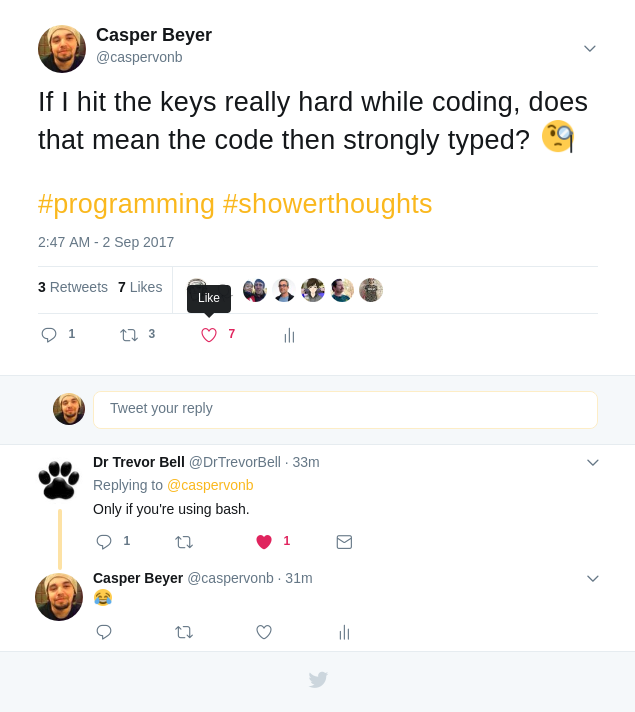
\includegraphics[width=.9\linewidth]{./images/strong-typing-twitter-meme.png}
\caption{Not what strongly typed means at all, but it is admittedly quite funny. (\citeprocitem{3}{Bayer, 2017})}
\end{figure}

 \newpage

For example, in Rust:
\begin{minted}[]{rust}
fn main() {

    // Create a floating point number
    let variable = 42.0;

    // Compare the floating point number
    // to an integer, which is a different type,
    // and check if they are the same
    let is_42 = 42.0 == 42;

    // Print whether the floating point number
    // is the same as the integer
    println!("The variable is 42: {}", is_42);
}
\end{minted}

In the above code, a floating point number
just means a number with decimal points.
An integer refers to a whole number,
which does not have decimal places.

 \newpage

Trying to compile the above code, which means
to turn the above code into machine code
that can run on your computer, results in
an error:
\begin{verbatim}
error[E0277]: can't compare `{float}` with `{integer}`
 --> src/main.rs:9:22
  |
9 |     let is_42 = 42.0 == 42;
  |                      ^^ no implementation for `{float} == {integer}`
  |
  = help: the trait `PartialEq<{integer}>` is not implemented for `{float}`
  = help: the following other types implement trait `PartialEq<Rhs>`:
            f128
            f16
            f32
            f64
            i128
            i16
            i32
            i64
          and 8 others

error[E0308]: mismatched types
 --> src/main.rs:9:25
  |
9 |     let is_42 = 42.0 == 42;
  |                         ^^ expected floating-point number, found integer

Some errors have detailed explanations: E0277, E0308.
For more information about an error, try `rustc --explain E0277`.
error: could not compile `playground` (bin "playground") due to 2 previous errors
\end{verbatim}

Why does this error occur? It is due to
Rust being strongly typed. In the above code,
Rust does not allow floating point numbers
to be converted to integers, and hence
it gives an error when compiling the code.

 \newpage

On the other hand, you have weakly typed languages like JavaScript,
which will implicitly convert variables of one type to another type
when performing operations on the variable.
So the example above written in JavaScript will run without any errors,
as shown below:
\begin{minted}[]{javascript}
// Create a floating point number
let variable = 42.0;

// Compare the floating point number
// to an integer, which is a different type,
// and check if they are the same
let is_42 = 42.0 == 42;

// Print whether the floating point number
// is the same as the integer
console.log(`The variable is 42: ${is_42}`);
\end{minted}

And the result:
\begin{verbatim}
The variable is 42: true
\end{verbatim}

Probably the most egregious and famous example of
JavaScript's weakly typed variables is the code below:
\begin{minted}[]{javascript}
console.log(("b" + "a" + + "a" + "a").toLowerCase());
\end{minted}

Which evaluates to something entirely unexpected:
\begin{verbatim}
banana
\end{verbatim}

\begin{figure}[htbp]
\centering

\includegraphics[scale=0.16]{./images/banana.jpg}
\caption{A banana! (\citeprocitem{22}{Migala, 2018})}
\end{figure}

 \newpage

Where did the two "n"s come from?
The reason is due to \texttt{+ "a"} in \texttt{+ + "a"}
being coerced to the string "NaN",
which stands for "not a number".
A string refers to a bunch of text,
usually enclosed in single ('') or
double quotes (""),
like "This is a string".
Hence, the result becomes:
\begin{minted}[]{javascript}
console.log(("b" + "a" + "NaN" + "a").toLowerCase());
\end{minted}

This kind of implicit conversion can cause bugs that
are extremely difficult to catch, as no errors are shown.
Instead, the expected output becomes malformed in a way
that doesn't make any sense, making it even more difficult
to debug and fix the problem. Programmers were so tired
of JavaScript's implicit conversion that the \texttt{===} operator
had to be added to JavaScript, which is the same as the \texttt{==}
equality operator, but without the type coercion that comes
with using \texttt{==} in JavaScript.  \\

The difference between the two equality operators can be seen below:
\begin{minted}[]{javascript}
console.log("0" == 0);   // Prints true
console.log("0" === 0);  // Prints false
\end{minted}

And the result:
\begin{verbatim}
true
false
\end{verbatim}

\begin{figure}[htbp]
\centering
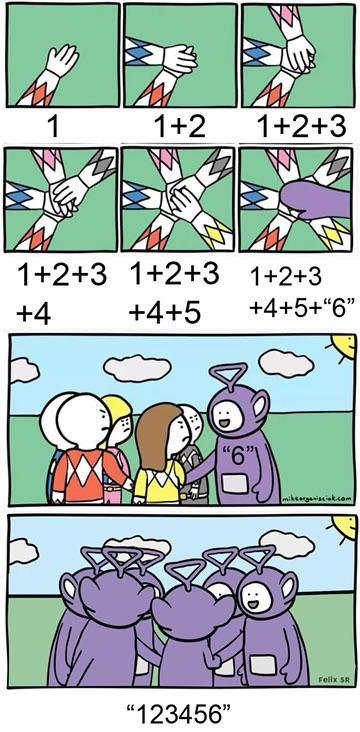
\includegraphics[scale=0.7]{./images/weak-typing-in-a-nutshell.jpg}
\caption{Weakly typed languages in a nutshell. (\citeprocitem{15}{GkAm1, 2021})}
\end{figure}

 \newpage

\subsection{Statically typed}
\label{sec:org8b22512}
A statically typed programming language is a programming language
that enforces variable types to remain the same throughout the whole program.
So let's say you create a new variable \texttt{foo} that is of the type \texttt{integer}.
For statically typed languages, after you have created that variable,
you are not allowed to change the type of
\texttt{foo} to a \texttt{string} afterwards.  \\

For example, in Rust:
\begin{minted}[]{rust}
fn main() {

    // Initialising a variable called foo of integer type
    let foo: i32 = 42;

    // Trying to change the variable foo to a string type
    foo = "string";
    println!("foo is: {}", foo);
}
\end{minted}

The above code won't compile,
and Rust will display a compilation error,
as shown below:
\begin{verbatim}
error[E0308]: mismatched types
 --> src/main.rs:7:11
  |
4 |     let foo: i32 = 42;
  |              --- expected due to this type
...
7 |     foo = "string";
  |           ^^^^^^^^ expected `i32`, found `&str`

For more information about this error, try `rustc --explain E0308`.
\end{verbatim}

 \newpage

On the other hand, you have dynamically typed programming languages,
like Python, which allow you to change the type of a variable
whenever you want. Hence, the code above written in Python would work
without any errors.
\begin{minted}[]{python}
# Initialising a variable called foo of integer type
foo = 42

# Changing the variable foo to a string type
foo = "string"
print(f"foo is: {foo}")
\end{minted}

\begin{verbatim}
foo is: string
\end{verbatim}


\begin{figure}[htbp]
\centering
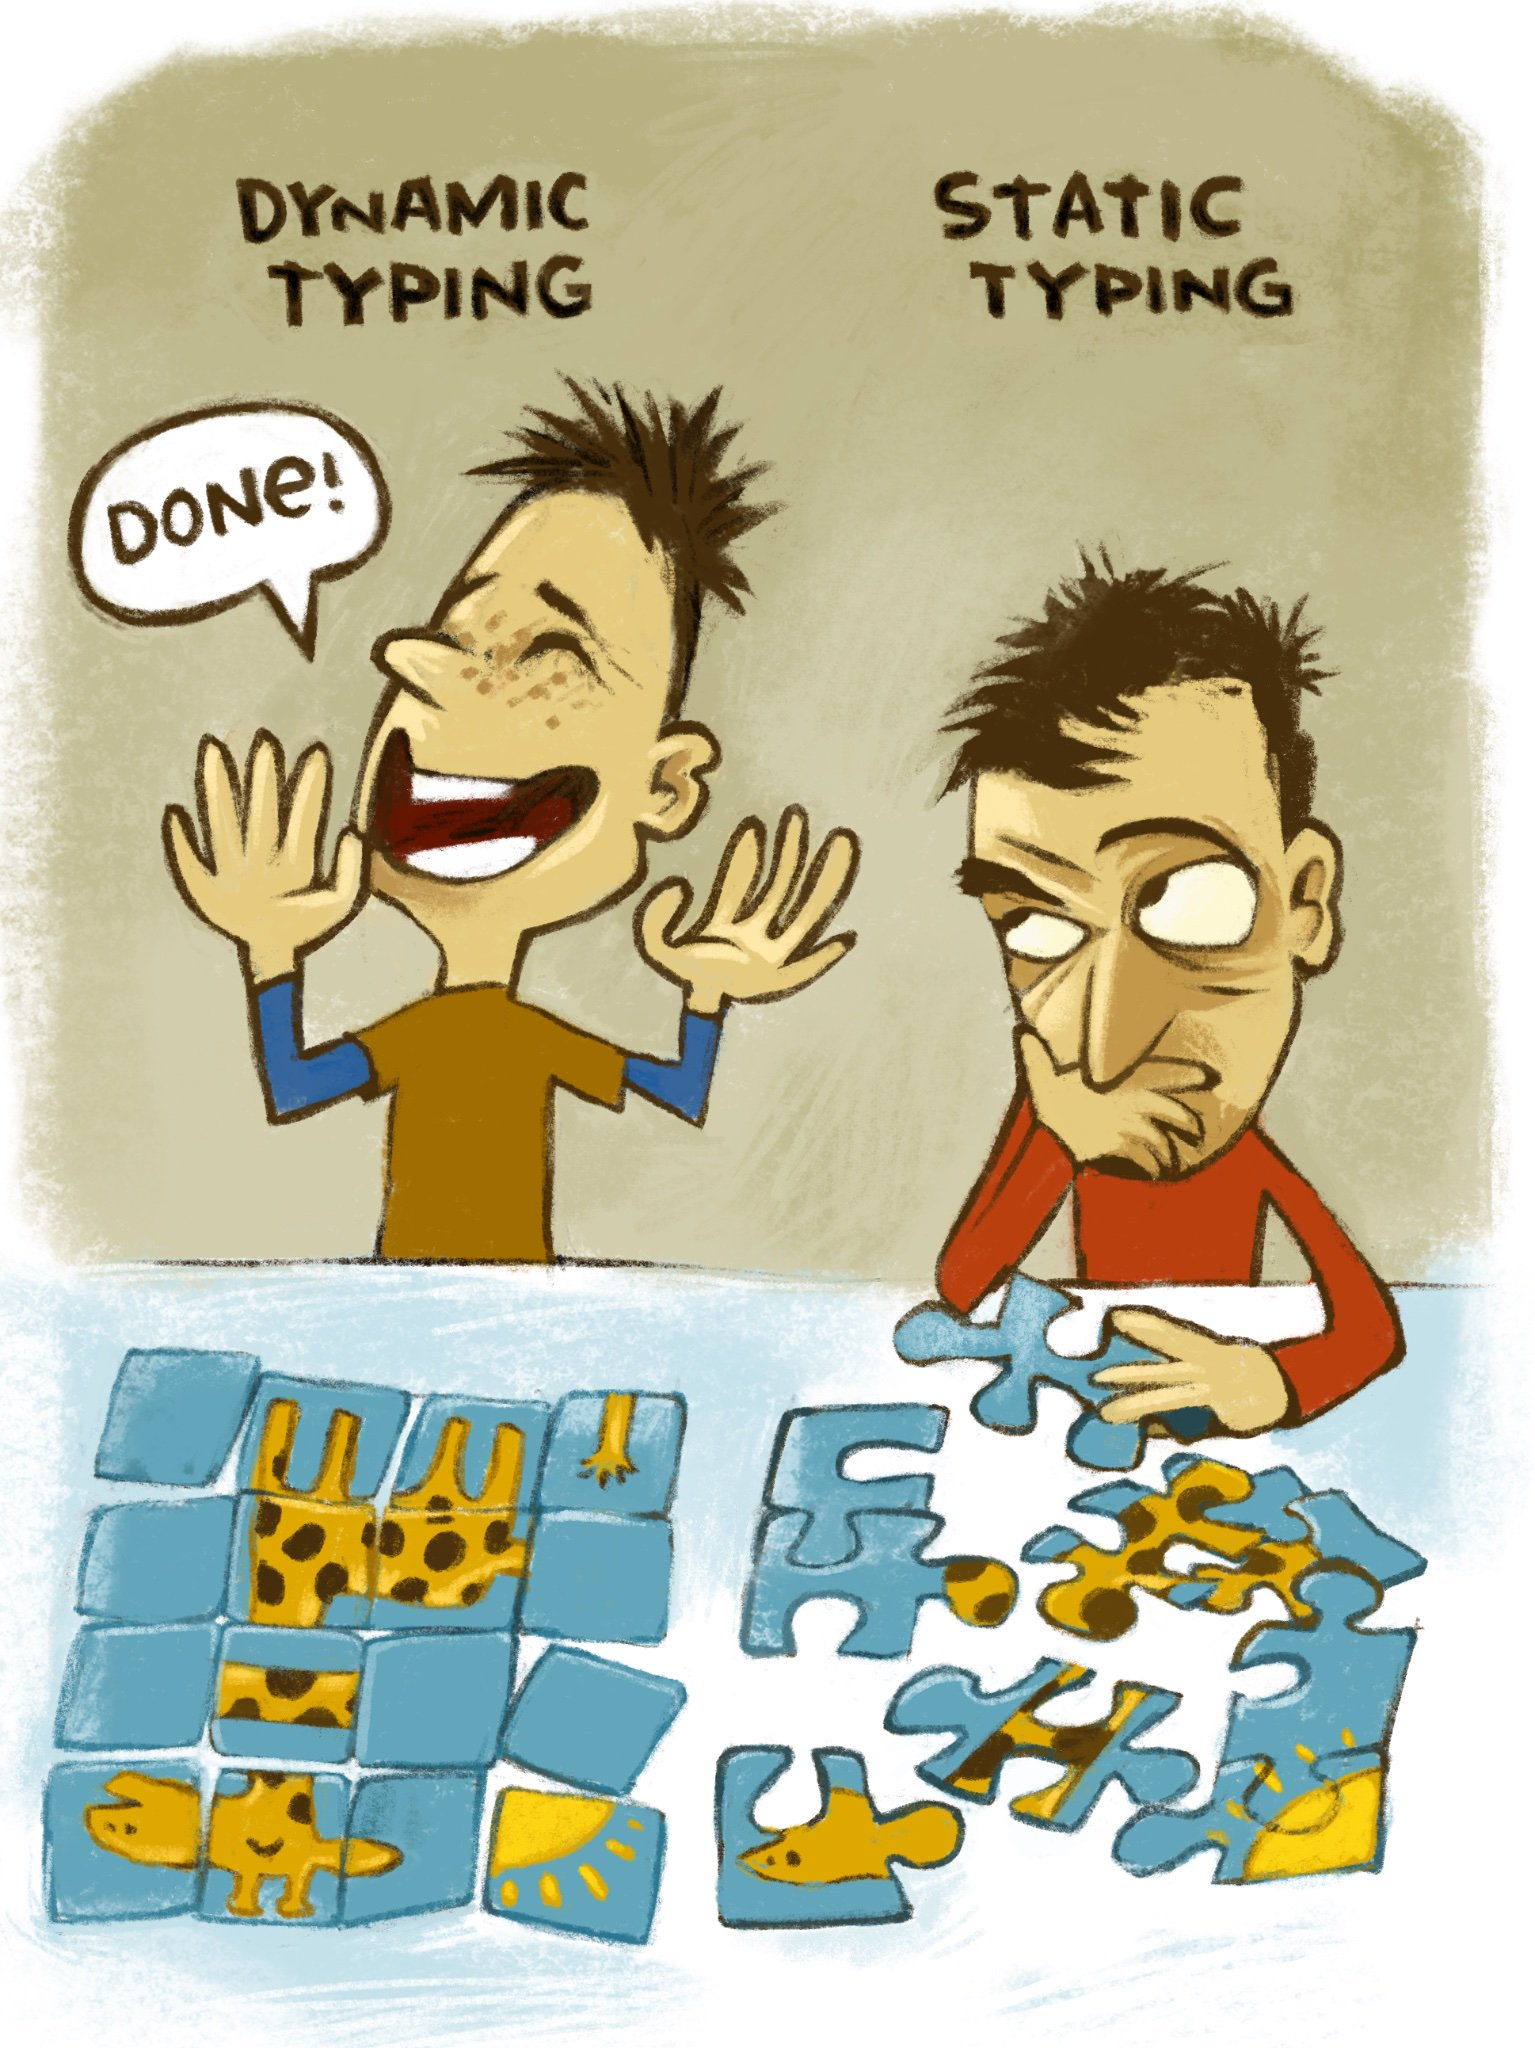
\includegraphics[scale=0.14]{./images/dynamic-vs-static-typing.png}
\caption{A meme about dynamic typing versus static typing. (\citeprocitem{46}{Wilcke, 2023})}
\end{figure}

\subsection{General-purpose}
\label{sec:org9811628}
A general-purpose programming language is a
programming language that can be used for most
programming tasks. Most popular programming languages,
like Python, Java and JavaScript can be used to make
almost anything you can think of. Usually, what makes
this easy to do is the existence of libraries.
Libraries are a collection of useful functions that make
it easier for you to write your program, as you don't
have to write everything yourself, you can instead
use what other people have written to save you time.
Functions are what you use in a programming language
to do something useful, and they usually receive inputs
and return an output. It also allows you to do the same
thing repeatedly without having to write the code
to do that thing over and over again.  \\

You can use Python to make games using the \href{https://www.pygame.org/news}{Pygame} library;
write basic servers using \href{https://flask.palletsprojects.com/en/3.0.x/}{Flask}; or complex web applications
using \href{https://www.djangoproject.com/}{Django}; do scientific computing with \href{https://numpy.org/}{Numpy},
\href{https://scipy.org/}{Scipy} and \href{https://matplotlib.org/}{Matplotlib}; write Telegram bots
with \href{https://pytba.readthedocs.io/en/latest/index.html}{pyTelegramBotAPI} and much more.
Similar libraries also exist for Java and JavaScript,
but I won't bore you by listing them all.  \\

Rust is also in the same vein, as you can create
games in Rust using the \href{https://bevyengine.org/}{Bevy game engine};
make Telegram bots using \href{https://github.com/teloxide/teloxide}{Teloxide}; create
web applications by compiling Rust code to something
called \href{https://webassembly.org/}{WebAssembly}, which by the way is an incredible piece
of technology that allows you to write web applications
in \textbf{any} programming language and
have it run in the browser. It is pure magic.  \\

Either way, you get the point, Rust can be used
to do whatever you want to do with it, and hence
it is considered a general-purpose programming language.

 \newpage

Programming languages that are not general-purpose
are considered domain-specific languages, or DSLs.
Some of the more prominent examples of DSLs include R
and Matrix Laboratory or MATLAB. These two languages
are mainly used for scientific computing and data analysis,
and aren't really suitable for other tasks.
Other DSLs include Structured Query Language (SQL),
which is used for reading, deleting and updating databases;
Hyper Text Markup Language (HTML), which is used to
display webpages on browsers;
Cascading Style Sheets (CSS), which is used to
beautify HTML webpages;
the Nix programming language,
which is a programming language to use to configure
a Nix Operating System (NixOS) and the
installation scripts for applications in NixOS;
and GNU Guile, which is also used for configuring
an operating system, namely the
GNU Guix System Distribution, and is also used
to define installation scripts for that system.

\begin{figure}[htbp]
\centering
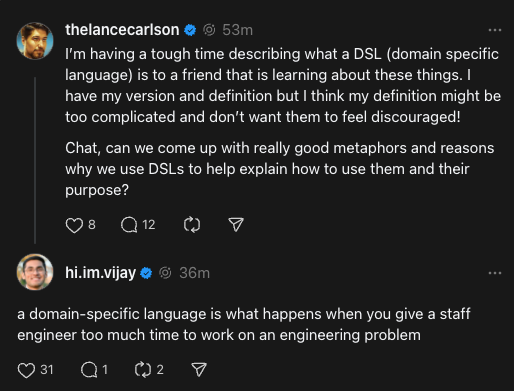
\includegraphics[width=.9\linewidth]{./images/domain-specific-languages.png}
\caption{Too true, this is just what happens most of the time. (\citeprocitem{42}{Vijay, 2024})}
\end{figure}

\section{What's so special about Rust?}
\label{sec:orgc60510b}
The three characteristics of Rust that I mentioned above
aren't unique to Rust. A lot of other programming
languages also possess the same three characteristics.
For example, Java, C, C++ and C\# are all general-purpose
programming languages that are statically and strongly typed.
What makes Rust special is its emphasis on performance,
type safety, concurrency and its enforcement of memory safety,
which caused the Rust language designers to do things
very differently.  \\

\begin{figure}[htbp]
\centering
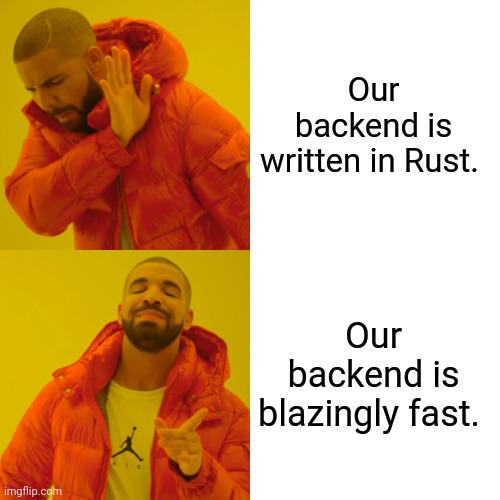
\includegraphics[height=29em]{./images/rust-is-blazingly-fast.jpeg}
\caption{Rust is indeed fast, thanks to its emphasis on performance. Read on to learn why! (\citeprocitem{12}{fnabinash, 2024})}
\end{figure}

Let's go over some of Rust's unique features.

\subsection{Errors as values}
\label{sec:orgdd90a76}
This feature of Rust is no longer unique in modern times,
as most recent programming languages have adopted errors
as values. But when compared to older programming languages
like Python, Java and JavaScript, which treat errors as
exceptional states (in Python and Java they are literally
called exceptions), it is much better.

\subsubsection{History of error handling}
\label{sec:orgd5094e6}
First, a bit of a history lesson. It is quite
funny how programmers have gone full circle
when it comes to error handling. Back in the 1970s and 1980s,
when C (\citeprocitem{29}{Ritchie, 1993}) and C++ (\citeprocitem{43}{Wikipedia, 2024a})
was one of the few programming languages around,
there was no concept of errors or exceptions,
and most programmers who used C and C++ returned integer codes
to indicate the state of the program. Exit codes are still
being used to this day, as most command line
(shell or terminal) utilities still use exit codes.
An exit code of \texttt{0} means the program ran
successfully without errors, while an exit code of \texttt{1}
means the program had an error while running. Other
exit codes are used to indicate other states of the program,
like specific error types and so on.  \\

This changed in the 1990s, with programming languages that
were created during that time, like Python (\citeprocitem{31}{Rossum, 1991})
and Java (\citeprocitem{4}{Binstock, 2015}), came with exceptions to
indicate error states instead of returning
exit codes or error values. This way of error handling continued
up until the 2010s, when new programming languages
such as Rust (\citeprocitem{44}{Wikipedia, 2024b}) and Zig (\citeprocitem{20}{Kelley, 2016})
and Go (\citeprocitem{45}{Wikipedia, 2024c}) treated errors as values instead
of treating errors as exceptions. Almost all new programming
languages treat errors as values in modern times, such
as Gleam.

 \newpage

Programmers have gone full circle from preferring errors
as values, to errors as exceptional states and back to
errors as values again. However, modern programming
languages that return errors as values no longer return
integer exit codes, but instead return descriptive errors.
These languages also include features to easily handle
these error values, like matching on the result of a
function to handle the result or the error, which is
definitely a huge upgrade from the integer exit codes
of the 1970s and 1980s.

\subsubsection{Treating errors as exceptions}
\label{sec:org382299b}
This form of error handling treats errors as exceptional states
in a program, meaning that errors are unexpected
and are considered special cases to handle.
Errors are considered the exception to the norm,
which results in error handling that uses a \texttt{try} and \texttt{catch} block.
When writing a program using a programming language that
treats errors as exceptions, you write the flow of the program
as though no errors will occur. Then, in places where
you expect errors to occur, you use a \texttt{try} and \texttt{catch} block
to handle the error. Inside the try block, you write the code
where you expect an error to occur. Inside the catch block,
you write the code to handle the error, like setting a variable
to its default value, printing out the error to notify the user
that an error has occurred, or outright crashing the program
if the error is irrecoverable. By default, programming languages
that treat errors as exceptions will automatically crash the
program when an error is encountered. When such programming languages
run your program, they "try out" the code you have written
in the \texttt{try} block, and if an error occurs,
it will execute the code you have written in the \texttt{catch} block
to handle the error.

 \newpage

Below is an example of a \texttt{try} and \texttt{catch} block in Python:
\begin{minted}[]{python}
# Initialise the number
number = 10

# Try block
try:

    # Get the result of dividing the number by 2
    result_1 = number / 2

    # Print out the result
    print("Dividing the number by 2:", result_1)

    # Get the result of dividing the number by 0
    result_2 = number / 0

    # Print out the result
    print("Dividing the number by 0", result_2)

# Catch block to catch the division by zero error
except ZeroDivisionError:
    print("Can't divide the number by 0!")
\end{minted}

\begin{verbatim}
Dividing the number by 2: 5.0
Can't divide the number by 0!
\end{verbatim}


\begin{figure}[htbp]
\centering
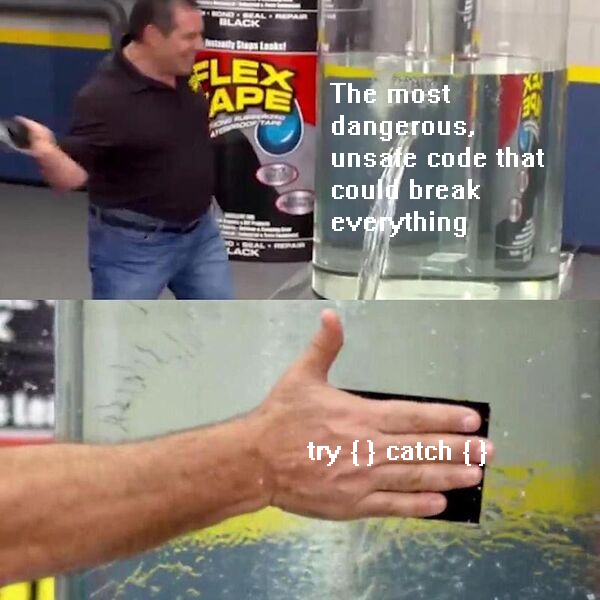
\includegraphics[width=.9\linewidth]{./images/try-catch-meme.png}
\caption{Ignore every error with exceptions! (\citeprocitem{39}{TheoXDM, 2022})}
\end{figure}

 \newpage

\subsubsection{Treating errors as values}
\label{sec:org7ec7037}
This form of error handling treats errors like any other
kind of value in a programming language.
Errors don’t cause a program to crash,
but instead just show up as a different value to handle.  \\

Below is the same example above written in Rust,
which treats errors as values:
\begin{minted}[]{rust}
fn main() {

    // Initialise the number
    let number: i32 = 10;

    // Get the result of dividing the number by 2
    let result_1 = i32::checked_div(number, 2);

    // Print out the result if it is not an error
    match result_1 {
        Some(result) => println!("Dividing the number by 2: {}", result),
        None => ()
    }

    // Get the result of dividing the number by 0
    let result_2 = i32::checked_div(number, 0);

    // Print out the result
    match result_2 {
        Some(result) => println!("Dividing the number by 0: {}", result),
        None => println!("Can't divide the number by 0!")
    }
}
\end{minted}

\begin{verbatim}
Dividing the number by 2: 5
Can't divide the number by 0!
\end{verbatim}

 \newpage

Treating errors as values does not necessarily mean that
the programming language has no way to crash the program
when there is an error. This is true of older
programming languages that treat errors as values like C and C++,
which will not crash until the program tries to access memory
it does not have access to, which is a memory access violation
called segmentation fault or segfault for short.
This error isn’t even caused by the programming language,
but instead caused by hardware that has memory protection.
Most modern programming languages that treat errors as values
provide a way to crash the program if an error is encountered,
usually by providing a function that crashes the program when used.  \\

Below is the same example above, still in Rust,
but I crash the program when an error occurs:
\begin{minted}[]{rust}
fn main() {

    // Initialise the number
    let number: i32 = 10;

    // Get the result of dividing the number by 2
    let result_1 = i32::checked_div(number, 2);

    // Print out the result
    println!("Dividing the number by 2: {}", result_1.unwrap());

    // Get the result of dividing the number by 0
    let result_2 = i32::checked_div(number, 0);

    // Print out the result
    println!("Dividing the number by 0: {}", result_2.unwrap());
}
\end{minted}

\begin{verbatim}
Dividing the number by 2: 5

thread 'main' panicked at src/main.rs:16:55:
called `Option::unwrap()` on a `None` value
note: run with `RUST_BACKTRACE=1` environment variable to display a backtrace
\end{verbatim}

\begin{figure}[htbp]
\centering

\includegraphics[width=.9\linewidth]{./images/dont-panic.jpg}
\caption{Keep calm, don't panic! Use the \texttt{Result} type instead. (\citeprocitem{30}{Rocha, 2018})}
\end{figure}

 \newpage

\subsubsection{Why is treating errors as values better?}
\label{sec:orgafd124f}
In programming languages that treat errors as exceptions,
the programmer can pretend that errors can’t happen in
their program and just have no error handling at all.
This is great for hastily written, one-time-use programs
as it allows such programs to be written in almost
no time at all. However, for complex programs that
need to be robust and fault-tolerant, treating
errors as exceptions is a bad idea.  \\

Programming languages that treat errors as exceptions
don't show errors in the function's signature.
A function's signature describes a function
in a programming language. It tells you the
parameters that you need to pass to the function,
that is, the input to the function, and the
return type of the function, which is the output
of the function.  \\

For example, here is a function that can fail in Python:
\begin{minted}[]{python}
def divide(divident: int | float, divisor: int | float) -> float:
    if divisor == 0:
        raise ZeroDivisionError
    return dividend / divisor
\end{minted}

The function's signature is the first line
starting with \texttt{def}. It tells you that
the function takes two integers or floating
point numbers, and returns a floating point
number. There is no mention of a possible
error that can occur when using the function,
which happens when the second number is 0.
This is important as you usually don't get
to look at the rest of the function below
the first line, also known as the body of the
function, or the implementation of the function.
Most of the time, you only see the function's
signature, and nothing else. For code that
is open-source, you can search their GitHub
repository for the implementation of the
function and figure out all the errors
that might occur when using the function.
However, for code that isn't open-source,
like a software development kit (SDK) provided
by Google for example, you have no idea
what errors can occur when using the function.

 \newpage

Not showing what errors a function can encounter
when it is being used makes it extremely difficult
to write robust and fault-tolerant programs, as you
will only know whether a function will crash the program
only when you run the program. For these kinds of
programming languages, the possible errors that can
occur is usually not well documented, so you will likely
be updating your program constantly for a while to
handle all the errors that your program encounters that
you have never anticipated. It is not a fun thing to do,
especially if you are working with a platform like Telegram
is always coming out with new features all the time,
which also means new error types to handle. Over time,
you would have encountered most of the possible errors
your program can encounter, so you no longer need to
update your program as often to handle errors.

\begin{figure}[htbp]
\centering

\includegraphics[height=28em]{./images/microsoft-edge-exception.png}
\caption{This is why you have errors as values. Disappointed in you, Microsoft. (\citeprocitem{36}{StBlaize, 2024})}
\end{figure}

 \newpage

On the other hand, programming languages that
treat errors as values force the programmer
to handle the errors, as there is no way to
avoid them and pretend that they don't exist,
since it is a possible output from a function.
Such languages also have errors as part of a function's
signature, as it is a return value, or an output,
of the function. This makes it easy to know which
functions can result in an error when used,
and hence programmers can handle these errors
appropriately in their code for the program.  \\

Here is an example of the above function in Rust,
which treats errors as values:
\begin{minted}[]{rust}
fn divide(divident: f32, divisor: f32) -> Result<f32, String> {
    if divisor == 0.0 {
        return Err(format!("Cannot divide {} by zero!", divisor));
    }
    return Ok(divident / divisor);
}
\end{minted}

From the function's signature, which is the first line
starting with \texttt{fn}, it tells us that the function takes
two floating point numbers and returns a \texttt{Result} type.
A \texttt{Result} type is a type that can either one of two values,
an \texttt{Ok} value, which is a floating point number (\texttt{f32}) and an
error \texttt{Err} value, which is a string (\texttt{String}).
We can tell immediately what functions in Rust can fail
just by looking at their signature and seeing if there
is a \texttt{Result} type being returned as the output of the function.
This is much better for creating robust and fault-tolerant programs
as we know what functions can fail, as well as how to handle
the errors.  \\

Knowing what errors can happen in a program before even running
the program allows programmers to make programs that don't have
to be fixed much when they are given to users, which makes the
user experience better and is more secure for users.
Users are less likely to encounter bugs that may compromise
their safety, security or privacy.

\begin{figure}[htbp]
\centering
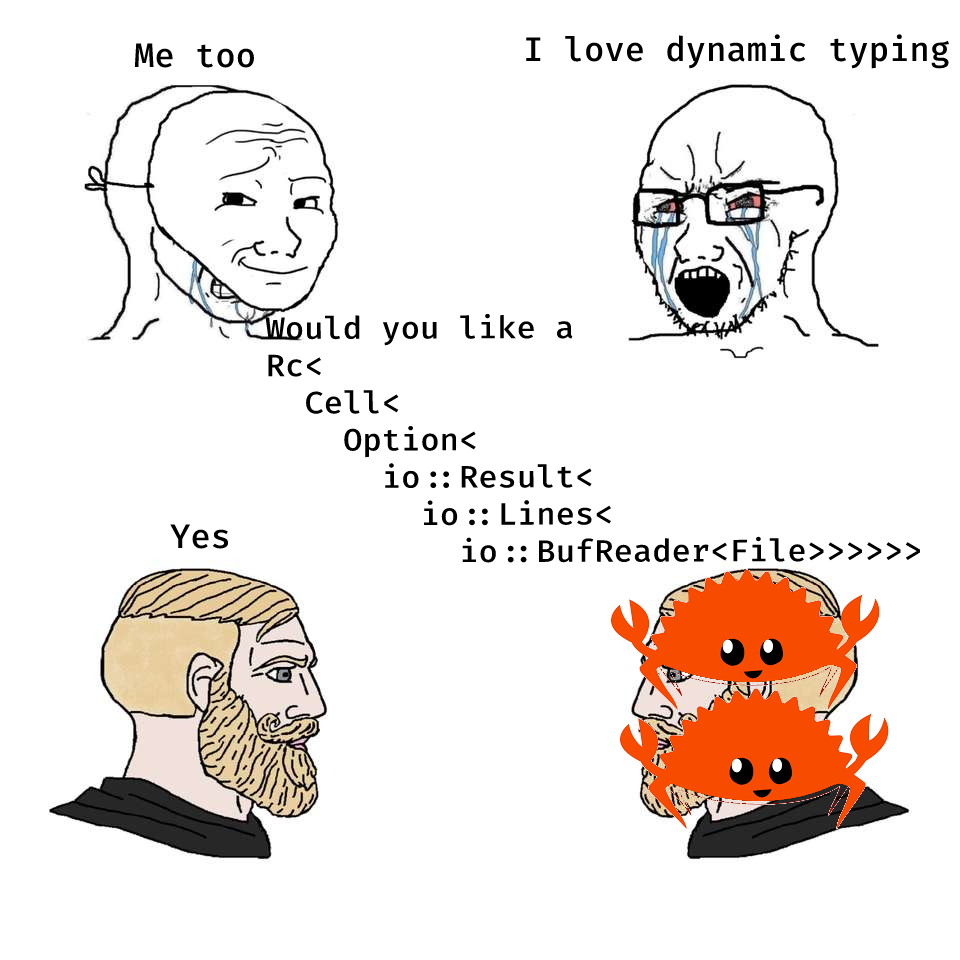
\includegraphics[width=.9\linewidth]{./images/return-types-in-rust.png}
\caption{Oops I think we went a bit too far here. (\citeprocitem{16}{GreekCSharpDeveloper, 2021})}
\end{figure}

 \newpage

\subsection{No garbage collector}
\label{sec:org292dcc3}
Garbage collector? In a programming language?
You mean programming languages also need a garbage man
to take out the trash?  \\

Yes, a garbage collector in a programming language
is pretty much the same as the garbage man coming
to your house to take out the trash. However,
instead of collecting actual garbage like your
garbage man does, the garbage collector in
a programming language collects
unused references to memory. Unused references to memory
in a programming language is essentially the programming
version of garbage, as they are no longer used and
are just taking up precious memory that other programs
on your computer want to use. Hence, they need to be collected,
cleaned up, and released so that other programs can use that
memory. Think of it like recycling, and the garbage collector
in a programming language is like the recycling man coming to
collect your recyclables to bring to the recycling plant to
recycle and create new materials, but instead of materials,
it is memory that it is creating.

\begin{figure}[htbp]
\centering

\includegraphics[height=20em]{./images/when-your-code-is-garbage.jpg}
\caption{When your code is garbage\ldots{} (\citeprocitem{2}{BabuShonaMuhMeLoNa, 2021})}
\end{figure}

 \newpage

\begin{figure}[htbp]
\centering
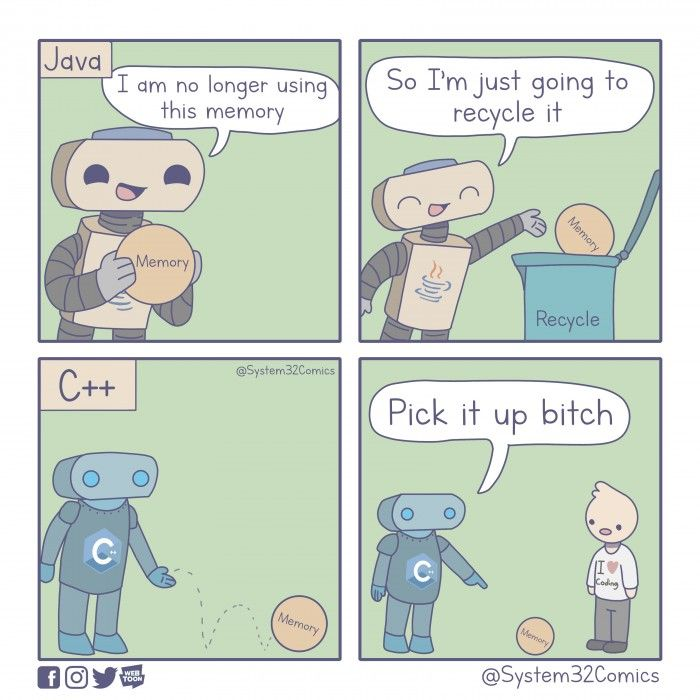
\includegraphics[width=.9\linewidth]{./images/garbage-collection.jpg}
\caption{Garbage collection (Java is a programming language with a garbage collector, while C++ doesn't have one) (\citeprocitem{13}{Forgotten\_Who, 2020})}
\end{figure}

 \newpage

\subsubsection{What's wrong with a garbage collector?}
\label{sec:org03a4148}
It seems like having a garbage collector in a programming
language is a good thing since it helps you clean up
and release the unused memory so that other programs
can use it. Otherwise, you would just run out of memory
storing useless information and crash your computer,
which would be absolutely terrible.  \\

However, you sacrifice performance by having a garbage
collector, because having someone to come collect your
garbage isn't free. You have to pay them to do so. In real life,
the government pays the garbage man a salary and you pay taxes
(you do right?). In a programming language,
it pays the cost of memory and CPU cycles,
which essentially means that the program is going to be slower
and use more memory because of garbage collection.
The garbage collector in a programming language is
separate process from the main program that needs to run when
the main program is running, which means it will take up
memory and use up CPU cycles that could have been used by
the program itself instead.  \\

Most of the time, this cost isn't much and shouldn't matter
for most programs. However, when it comes to performance
critical applications, like trading bots or servers
like Google handling massive amounts of web traffic every day,
this performance cost adds up to a hefty amount, so it makes
sense to not use a garbage collector in such situations.

\begin{figure}[htbp]
\centering

\includegraphics[height=14em]{./images/cpp-being-garbage.jpg}
\caption{Throwing shade at C++. (\citeprocitem{5}{Bit48, 2021})}
\end{figure}

 \newpage

\subsubsection{Freeing memory manually}
\label{sec:org040810f}
Well, if I don't want to pay someone to help me take out the trash,
then I'll have to do it myself. This is exactly what low-level
programming languages, which are programming languages
that allow you to manipulate memory directly, like C and C++, do.
You will have to take out the trash by yourself, manually.
What this means is that you will have to free the unused
memory yourself.  \\

Below is an example of that in C:
\begin{minted}[]{c}
#include <stdlib.h>

int main() {

  // Allocate memory for a string of 10 characters
  char *string = malloc(10 * sizeof(char));

  // If the memory has not been allocated,
  // exit the program
  if (string == NULL) exit(1);

  // Free the memory
  free(string);

  // Return zero
  return 0;
}
\end{minted}

 \newpage

\begin{figure}[htbp]
\centering

\includegraphics[height=36em]{./images/clean-up-after-yourself.jpg}
\caption{Clean up after yourself, please. (\citeprocitem{18}{ItsCaptainS, 2022})}
\end{figure}

\subsubsection{What's wrong with freeing memory manually?}
\label{sec:orgf53904c}
It seems like freeing memory isn't too difficult to do,
you just need to remember that you allocated memory for
a variable and then free it afterwards.

 \newpage

Turns out that in reality, that is absolutely not the case at all.
In the simple example I showed above, it is trivial to remember
to free the memory since there is only one variable to keep track of.
However, in programs that are thousands, or even hundreds of thousands
to millions of lines of code long, there is just no way anyone
can keep track of all the variables that have memory allocated to them
and hence need to be freed. It is just impossible to do. It is the
reason why the garbage collector was created in the first place,
so that programmers don't have to manually free the memory that they use
as it is a massive inconvenience and can lead to a lot of bugs.  \\

One type of bug is the use-after-free bug, which is when you use
a variable after you have freed the memory for it.  \\

Below is an example in C:
\begin{minted}[]{c}
#include <stdlib.h>
#include <stdio.h>

int main() {

  // Allocate memory for a string of 10 characters
  char *string = malloc(10 * sizeof(char));

  // If the memory has not been allocated,
  // exit the program
  if (string == NULL) exit(1);

  // Free the memory
  free(string);

  // Print the string after freeing memory.
  // Use-after-free bug.
  printf(string);

  // Return zero
  return 0;
}
\end{minted}

 \newpage

\begin{figure}[htbp]
\centering
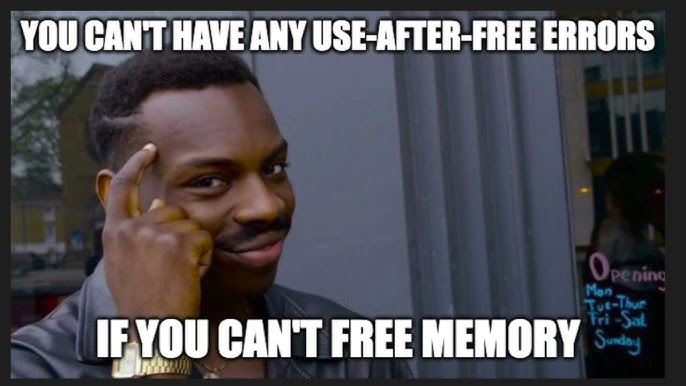
\includegraphics[width=.9\linewidth]{./images/use-after-free-bugs.jpg}
\caption{Well he's not wrong, and that's exactly the approach Rust takes. (\citeprocitem{35}{Skills, 2022})}
\end{figure}

 \newpage

Another type is a double-free bug, which is when you
free the memory for a variable twice, usually by accident.  \\

\begin{listing}[htbp]
\begin{minted}[]{c}
#include <stdlib.h>
#include <stdio.h>

int main() {

  // Allocate memory for 2 integers
  int* pointer_to_int_1 = (int*) malloc(sizeof(int));
  int* pointer_to_int_2 = (int*) malloc(sizeof(int));

  // Set the first integer to 10
  *pointer_to_int_1 = 10;

  // Set the second integer to 20
  *pointer_to_int_2 = 20;

  // Set the pointer to the first integer
  // to the pointer to the second integer
  pointer_to_int_1 = pointer_to_int_2;

  // Print out the two integers
  printf("%d %d", *pointer_to_int_1, *pointer_to_int_2);

  // Free the memory used for both integers
  free(pointer_to_int_1);
  free(pointer_to_int_2);

  // Return zero
  return 0;
}
\end{minted}
\caption{The code above is an example in C.}
\end{listing}
\label{org3c03684}

You might be asking how there is a double-free bug in the above code,
since both \texttt{pointer\_to\_int\_1} and \texttt{pointer\_to\_int\_2} seem to be two
different variables and hence are freed separately.

 \newpage

The main issue with the above code is the line
\texttt{pointer\_to\_int\_1 = pointer\_to\_int\_2}, which sets
the variable storing the pointer to the first integer
to store the pointer to the second integer instead.
Now the \texttt{pointer\_to\_int\_1} variable is referring
to the same memory location as \texttt{pointer\_to\_int\_2},
so \texttt{free(pointer\_to\_int\_1)} frees the memory used
by \texttt{pointer\_to\_int\_2}. The next line,
\texttt{free(pointer\_to\_int\_2)} also
frees the memory used by \texttt{pointer\_to\_int\_2},
causing a double-free bug.

\begin{figure}[htbp]
\centering
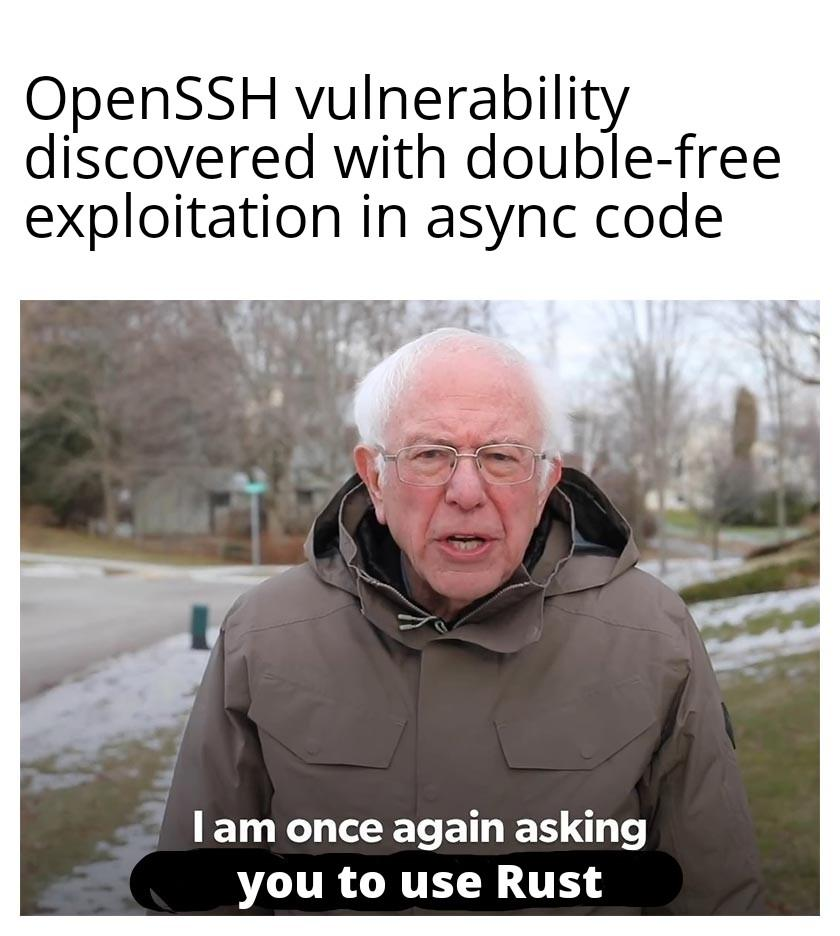
\includegraphics[width=.9\linewidth]{./images/double-free-bugs.jpeg}
\caption{People please, use Rust. (\citeprocitem{7}{ChipNDipPlus, 2024b})}
\end{figure}

 \newpage

There is also one more type of bug present in the code above,
and it is called a memory leak. A memory leak is when a program
uses some memory and fails to release the memory it used when it
is done with it. This results in the program hogging memory that
it doesn't need, as it is already done using the memory, but just
failed to release it back to the system. It is called a "leak"
as the program no longer has any control over the memory that it
is done with and was supposed to release back to the system.
The program can't even release the memory back to the system
even if it wanted to, because it has lost track of that memory.
Hence, that memory "leaks" into the system. As the program
continues the run, it will hog more and more memory,
decreasing the amount of available memory on the system until
it eventually hogs all the memory that the system has,
and causes the system to crash due to running out of memory.  \\

You can think of memory leaks like borrowing a book from the library,
but failing to return the book because you lost it. You start by
borrowing a few books from the library, but every time you return the
books to the library, you lose one book. As time passes, the library
starts to have fewer available books for you to borrow
because you lose a book every time you borrow books from the library.
Eventually, the library runs out of books and has to shut down.

\begin{figure}[htbp]
\centering

\includegraphics[height=15em]{./images/memory-leak-humans-vs-computers.jpg}
\caption{Another way to think about memory leaks. (\citeprocitem{27}{OOLarge, 2019})}
\end{figure}

 \newpage

Memory leaks are extremely difficult bugs to catch and debug due
to their subtlety. They are not obvious and usually have
very minimal impact on the system until it causes the system
to run out of memory entirely and crash. This usually only
happens after running the program for a very long time, and hence
nothing happens most of the time. It is a silent killer, you only
know something is wrong when your computer has already crashed.

\begin{figure}[htbp]
\centering
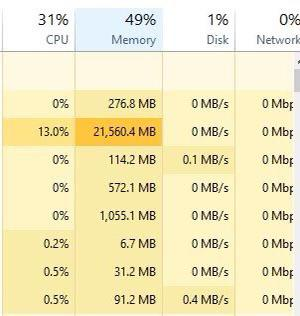
\includegraphics[width=.9\linewidth]{./images/my-program-has-a-memory-leak.jpg}
\caption{Did you say my program has a memory leak? (\citeprocitem{38}{TheONEO, 2021})}
\end{figure}

 \newpage

Back to the code \hyperref[org3c03684]{above}, if you have thought
about it intently, you would have noticed that the
program does indeed lose track of the memory
allocated to the \texttt{pointer\_to\_int\_1} variable initially.
When the line \texttt{pointer\_to\_int\_1 = pointer\_to\_int\_2}
is executed, the program no longer has a reference
to the memory allocated to the initial \texttt{pointer\_to\_int\_1}
variable, as now the \texttt{pointer\_to\_int\_1} variable
points to the memory used by the \texttt{pointer\_to\_int\_2}
variable. The memory used by the \texttt{pointer\_to\_int\_1}
is now inaccessible by the program and is hence lost.
The program can't free the memory used by the
initial \texttt{pointer\_to\_int\_1} variable as there is nothing
referring to it. Remember that the \texttt{free(pointer\_to\_int\_1)}
frees the memory used by the \texttt{pointer\_to\_int\_2} variable,
not the initial \texttt{pointer\_to\_int\_1} variable.
So the memory used by the initial \texttt{pointer\_to\_int\_1}
variable has leaked into the system, which is a memory leak.

\subsubsection{Ownership and borrowing}
\label{sec:orgd46a3bc}
The Rust language designers did not want to use a garbage collector,
as it sacrifices performance, but at the same time also wanted
to ensure memory safety. Allowing the programmer to manually manage
memory is powerful, but as Spider-Man says,
"With great power comes great responsibility",
the programmer is responsible for managing their memory properly,
which is a huge responsibility that not many can take up.
In fact, too many programmers today have failed to fulfil
their responsibility of managing memory properly.
It is also way too easy for programmers to write code that
creates memory-related bugs, like the aforementioned use-after-free,
double-free and memory leak bugs. It is much better to completely
eliminate the class of memory-related bugs by ensuring memory safety
in Rust. Hence, the Rust language designers came up with the brilliant
concept of ownership and borrowing in Rust to ensure memory safety
while remaining performant by not using a garbage collector.  \\

 \newpage

Ownership and borrowing in Rust work exactly as you would expect.
Whenever you create a variable with an initial value, that variable
"owns" the value. A value can only have one singular "owner".
When you want to set another variable to the same
value, the new variable can either "borrow" the value from the first
variable, or "take" the value from the first variable.

\begin{figure}[htbp]
\centering
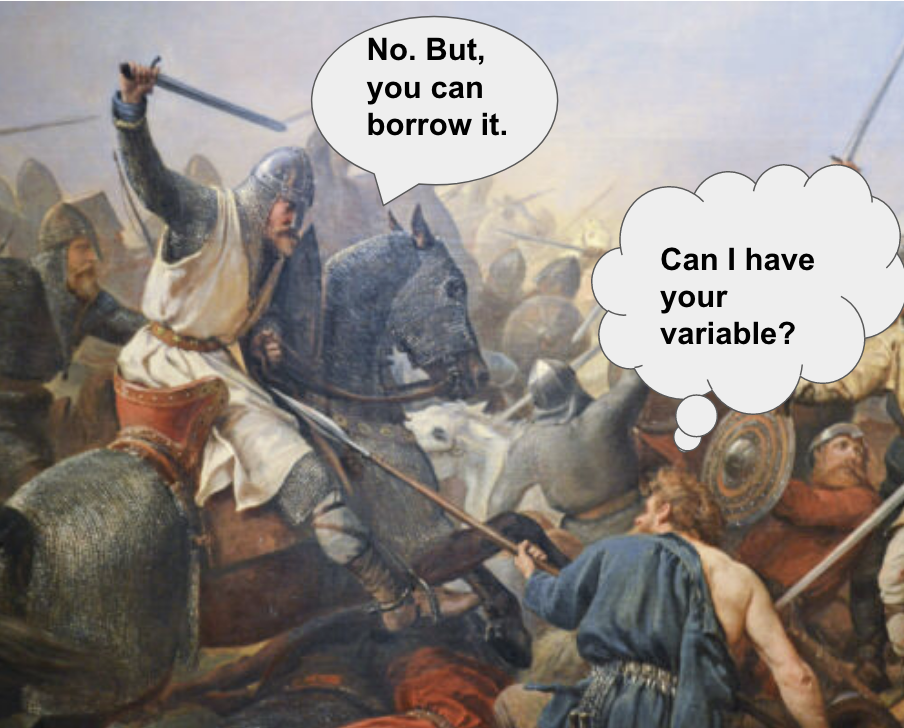
\includegraphics[width=.9\linewidth]{./images/ownership-and-borrowing.png}
\caption{Ownership and borrowing. (\citeprocitem{10}{Daniel, 2023})}
\end{figure}

 \newpage

In the former case where the new variable
"borrows" the value from the initial variable:
\begin{minted}[]{rust}
fn main() {

    // Initialise a variable with a value of "Hello".
    // The variable "string" owns the value of "Hello".
    let string = String::from("Hello");

    // Borrowing the value from the string variable
    let new_string = &string;

    // Print the string and the new string
    println!("string is: {}", string);
    println!("new_string is: {}", new_string);
}
\end{minted}

\begin{verbatim}
string is: Hello
new_string is: Hello
\end{verbatim}

You may notice that the symbol to "borrow"
the value from the string variable is an
ampersand (\texttt{\&}), which is the same as C's
symbol for "memory address of". It tells you
that the \texttt{new\_string} variable just refers
to the address of the \texttt{string} variable
for its value. Basically, the \texttt{new\_string}
variable is a reference to the \texttt{string} variable.
That is what "borrowing" is in Rust, a reference
to another variable.

 \newpage

In the latter case where the new variable
"takes" the value from the initial variable:
\begin{minted}[]{rust}
fn main() {

    // Initialise a variable with a value of "Hello".
    // The variable "string" owns the value of "Hello".
    let string = String::from("Hello");

    // Taking the value from the string variable
    // The variable "new_string" now owns the value of "Hello"
    let new_string = string;

    // Print the string and the new string
    println!("string is: {}", string);
    println!("new_string is: {}", new_string);
}
\end{minted}

 \newpage

And it doesn't compile:
\begin{verbatim}
error[E0382]: borrow of moved value: `string`
  --> src/main.rs:11:31
   |
5  |     let string = String::from("Hello");
   |         ------ move occurs because `string` has type `String`,
   |                which does not implement the `Copy` trait
...
8  |     let new_string = string;
   |                      ------ value moved here
...
11 |     println!("string is: {}", string);
   |                               ^^^^^^ value borrowed here after move
   |
   = note: this error originates in the macro `$crate::format_args_nl`
     which comes from the expansion of the macro `println`
     (in Nightly builds, run with -Z macro-backtrace for more info)
help: consider cloning the value if the performance cost is acceptable
   |
8  |     let new_string = string.clone();
   |                            ++++++++

For more information about this error, try `rustc --explain E0382`.
error: could not compile `playground` (bin "playground") due to 1 previous error
\end{verbatim}

Why does it not compile? Because the \texttt{new\_string} variable
has "taken" the value of \texttt{Hello} from the \texttt{string} variable,
which means the \texttt{string} variable now has nothing,
so it is removed and the memory it uses is cleaned up immediately.
This is called moving in Rust, as the \texttt{string} variable is
literally moved into the \texttt{new\_string} variable,
so it doesn't exist any more. You can't print
something that doesn't exist, so the program doesn't compile.

 \newpage

How does this ensure memory safety? Well, by using the concept
of ownership, it is easy for Rust to determine whether a variable
is still being used or not. When a variable is not a reference,
and no longer "owns" any value, the memory used by the variable
is automatically freed. You no longer need to manually free
the memory used by a variable. Then, the Rust compiler prevents you
from using or referring to variables that have their memory freed,
preventing the aforementioned use-after-free and double-free bugs.
For variables that don't have their values "taken" by another
variable, the memory used by it is automatically freed once
the variable goes out of scope. A scope in Rust is basically
the code inside a pair of curly braces (\texttt{\{\}}) that is not
inside single ('') or double quotes ("").
This way, there are no memory-related bugs that can occur
and no memory leaks as all the memory used is being freed,
and all of it is automatic. It looks like we can have our
cake and eat it too.  \\

There are more rules to Rust's system of ownership and
borrowing which is enforced by a system in Rust called
the borrow checker, but the rest are not very relevant,
so I shall not bore you with the details.

\begin{figure}[htbp]
\centering

\includegraphics[height=21em]{./images/rust-borrow-checker-in-a-nutshell.png}
\caption{Life is hard when you write Rust. (\citeprocitem{41}{valchap, 2023})}
\end{figure}

 \newpage

\subsection{Explicit mutability}
\label{sec:orgc63c1e8}
Explicit mutability means that you have to explicitly
state that you want something to change for it to change.
In the programming context, this refers to the ability
of variables to change. In most programming languages,
variables are implicitly mutable, which means they
can change by default. This makes sense, especially
considering the meaning of the word "variable",
as it refers to something that can vary or change.
However, in Rust, variables are implicitly immutable,
which means that they cannot be changed by default.
You will have to explicitly mark a variable as
mutable by using the keyword \texttt{mut}.  \\

For example:
\begin{minted}[]{rust}
let mut number = 1;
\end{minted}

Trying to change a variable without marking it
as mutable beforehand will cause the program
to not compile:
\begin{minted}[]{rust}
fn main() {
    let number = 1;
    number = 2;
    println!("number is: {}", number);
}
\end{minted}

 \newpage

And the error:
\begin{verbatim}
error[E0384]: cannot assign twice to immutable variable `number`
 --> src/main.rs:3:5
  |
2 |     let number = 1;
  |         ------ first assignment to `number`
3 |     number = 2;
  |     ^^^^^^^^^^ cannot assign twice to immutable variable
  |
help: consider making this binding mutable
  |
2 |     let mut number = 1;
  |         +++

For more information about this error, try `rustc --explain E0384`.
error: could not compile `playground` (bin "playground") due to 1 previous error
\end{verbatim}

Let's fix the above code by marking the
\texttt{number} variable as mutable with the \texttt{mut}
keyword:
\begin{minted}[]{rust}
fn main() {
    let mut number = 1;
    number = 2;
    println!("number is: {}", number);
}
\end{minted}

\begin{verbatim}
number is: 2
\end{verbatim}

When variables being mutable is the default,
it is very easy to accidentally change the
value of a variable without realising that
you have changed it, either through a typo
when typing the variable name, or just
mistaking a variable for another one.
Mistakes like this happen all the time
and are the cause of a lot of headaches
for programmers. Rust helps you write
less buggy code by forcing you to
explicitly mark mutable variables
so that you know where to look when
something doesn't go right with your program.
This makes it easier for programmers to locate,
debug and fix bugs, making programs written
in Rust more robust and error-free.

\begin{figure}[htbp]
\centering

\includegraphics[width=.9\linewidth]{./images/pronunciation-of-mut.jpg}
\caption{How do you pronounce \texttt{mut}? (\citeprocitem{34}{SirKastic23, 2023})}
\end{figure}

\subsection{Unsafe keyword}
\label{sec:org05a0301}
The \texttt{unsafe} keyword in Rust allows you to perform
direct memory manipulation like you can with C and
C++, and also allows Rust code to make use of external code,
usually written in C or C++ without the Rust compiler constantly
screaming about errors that are impossible to fix.
The compiler is a program that turns the code you
write into machine code that can run on your computer.
This gives advanced programmers who know what they are
doing the power to do what they need to do, which is
usually optimisation of a program. This keyword
doesn't disable all checks by the Rust compiler,
so you don't have the freedom to do absolutely whatever
you want to do like you have in C and C++, but
allows you to do some things that are normally
prohibited by the Rust compiler, like make use
of \texttt{unsafe} functions, or use external code.  \\

\begin{figure}[htbp]
\centering

\includegraphics[width=.9\linewidth]{./images/unsafe-to-go-alone.png}
\caption{Aww, thanks Ferris. (Ferris is Rust's mascot, the crab.) (\citeprocitem{23}{mottosson, 2021})}
\end{figure}

The main reason behind the \texttt{unsafe} keyword is
that it allows Rust to use functions from other
programming languages inside Rust, most notably
C and C++. Because there has already been so much
code written in C and C++, a lot of programmers that
use Rust want to make use of that code to make
writing their programs easier, so the \texttt{unsafe}
keyword helps these programmers integrate Rust
into their ecosystem without needing to rewrite
every single thing in Rust. They can slowly
rewrite parts of their ecosystem to Rust
and still have everything working as usual.
This feature of Rust can be considered a
necessity for it to gain traction and
popularity among programmers, as having
to rewrite all existing code in Rust
is a massive undertaking, and an
incredibly tedious and arduous process.
The reason for marking external code as
unsafe is that pretty much all other
programming languages lack the safety guarantees that
Rust provides, and the \texttt{unsafe} keyword
makes that immediately obvious.
It also makes it obvious as to where
memory-related bugs can originate from,
as it marks a block of code as unsafe,
making it easier to locate, debug
and fix bugs.

 \newpage

Below is a simple example of
the \texttt{unsafe} keyword in Rust:
\begin{minted}[]{rust}
fn main() {

    // Create a number
    let number = 1;

    // Create a raw immutable pointer to the number
    let raw_pointer_to_number = &number as *const i32;

    // Unsafe block, as dereferencing a raw
    // pointer is considered unsafe
    unsafe {

        // Print out the value of the number
        // by dereferencing the raw pointer
        println!("number is: {}", *raw_pointer_to_number);
    }
}
\end{minted}

\begin{verbatim}
number is: 1
\end{verbatim}

This feature does not make Rust more memory-safe,
in fact, it makes Rust memory unsafe, because
memory safety isn't guaranteed inside
unsafe blocks, and you as the programmer
have to ensure that memory safety is guaranteed
inside \texttt{unsafe} blocks. This feature exists
to make it much easier to use Rust for
whatever you want to do, and to make
the transition from languages like
C and C++ to Rust smoother, improving
the experience for programmers. After all,
if we want people to write their programs
in Rust, we need to make it easy for them
to do so right?

\begin{figure}[htbp]
\centering

\includegraphics[width=.9\linewidth]{./images/what-it-feels-like-to-use-unsafe.jpg}
\caption{Footgun unlocked, get ready for pain! (\citeprocitem{9}{corianderL, 2020})}
\end{figure}

 \newpage

\section{Benefits of Rust}
\label{sec:orgd2312d3}
The main benefits of Rust are its emphasis on
performance while enforcing memory safety
(all bets are off if you use the \texttt{unsafe}
keyword though). This allows programmers to
create robust and fault-tolerant programs that
is free of memory-related bugs such as the
aforementioned use-after-free, double free
and memory leak bugs. This eliminates an
entire class of memory bugs that are
just simply impossible to encounter when
using Rust to write your programs, which
would make your program far safer by default
when compared to the same program written
in C or C++.  \\

In Rust, there is also a huge emphasis on the
correctness of a program, and the language
features are designed in such a way that
makes it more difficult to write incorrect code.
For example, Rust requires you to represent
all possible states in your program as a type,
usually in something called an enumeration,
or enum for short. An enumeration is just a
set of values with names to easily refer to
the value. Enumerations are also usually grouped
together, which makes it very useful for \texttt{match}
statements in Rust, where you match against
the values of an enumeration to decide
what to do with the value.

\begin{center}
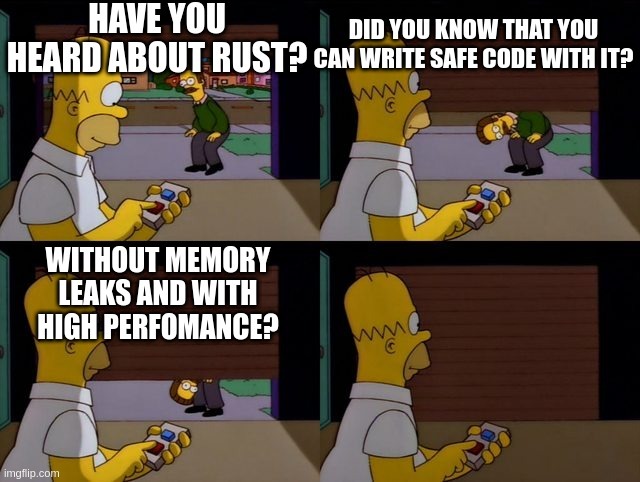
\includegraphics[height=18em]{./images/benefits-of-rust.png}
\captionof{figure}{Rust developers can sometimes evangelise about the benefits of Rust a bit too much. (\citeprocitem{25}{navierstokes88, 2023})}
\end{center}

 \newpage

Below is an example of matching against
enumerations in Rust:
\begin{minted}[]{rust}
fn main() {

    // Initialise a list of numbers
    let number_list = [10, 20, 30];

    // Get a number from the list
    let number = number_list.get(0);

    // If the number exists, print it out.
    // Otherwise, print that the index is out of bounds.
    match number {
        Some(value) => println!("number is: {}", value),
        None => println!("The index is out of bounds of the list.")
    }
}
\end{minted}

\begin{verbatim}
number is: 10
\end{verbatim}

Rust makes heavy use of matching a value against
an enumeration, as enumerations are exhaustive
and will force programmers to consider all cases,
instead of just one case, which reduces the number
of bugs in a program.  \\

Let's see what happens if I don't handle all cases
of the enumeration in the above example:
\begin{minted}[]{rust}
fn main() {

    // Initialise a list of numbers
    let number_list = [10, 20, 30];

    // Get a number from the list
    let number = number_list.get(0);

    // If the number exists, print it out.
    match number {
        Some(value) => println!("number is: {}", value)
    }
}
\end{minted}

 \newpage

\begin{verbatim}
error[E0004]: non-exhaustive patterns: `None` not covered
   --> src/main.rs:11:11
    |
11  |     match number {
    |           ^^^^^^ pattern `None` not covered
    |
note: `Option<&i32>` defined here
   --> /playground/.rustup/toolchains/stable-x86_64-unknown-linux-gnu/lib/
    |  rustlib/src/rust/library/core/src/option.rs:574:1
    |
574 | pub enum Option<T> {
    | ^^^^^^^^^^^^^^^^^^
...
578 |     None,
    |     ---- not covered
    = note: the matched value is of type `Option<&i32>`
help: ensure that all possible cases are being handled by adding
a match arm with a wildcard pattern or an explicit pattern as shown
    |
12  ~         Some(value) => println!("number is: {}", value),
13  +         None => todo!()
    |

For more information about this error, try `rustc --explain E0004`.
error: could not compile `playground` (bin "playground") due to 1 previous error
\end{verbatim}

Expectedly, the program doesn't compile and the Rust
compiler tells me to add a match arm for the \texttt{None} type.
This forces me to handle all possible cases instead of
just assuming that I will be able to get the number
out of the list, resulting in fewer bugs and a more
robust and fault-tolerant program.

 \newpage

\begin{center}
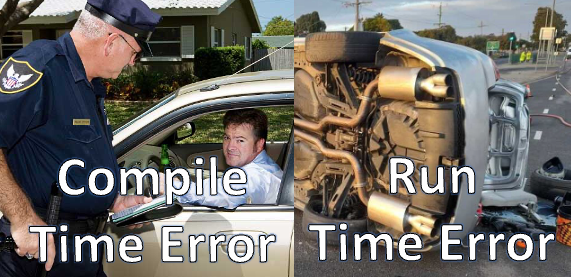
\includegraphics[width=.9\linewidth]{./images/compile-time-vs-run-time-error.png}
\captionof{figure}{Catching bugs when you are compiling the program is much better than catching bugs when the program is running. (\citeprocitem{11}{ElyeProj, 2022})}
\end{center}

\begin{center}

\includegraphics[height=26em]{./images/helpful-rust-compiler.png}
\captionof{figure}{Not to mention that the compiler is super helpful too! (\citeprocitem{21}{LinearArray, 2024})}
\end{center}

 \newpage

\section{Cons of Rust}
\label{sec:orgde300d1}
The biggest cons with using Rust is probably its
development time and the difficulty of the programming
language. I will also cover some other cons
that are relatively minor compared to the two
mentioned above.

\subsection{Longer development time}
\label{sec:org7ce3b72}
With Rust being so strict about everything and
forcing you to make sure that you have accounted
for every single case, it makes it far longer to
get a program that will actually get through
the Rust compiler compared to other programming
languages. This makes Rust a subpar language for
hastily written prototypes and proof of concepts,
as it takes far too long to develop those in Rust.
Rust does have a few features to help with these
kinds of fast iteration, like the \texttt{unwrap} function
on the \texttt{Option} enumeration to simply crash
the program if the value contained in the \texttt{Option}
enumeration is \texttt{None} instead of \texttt{Some}. It allows
you to pretend that errors don't exist, similar
to languages that treat errors as exceptions, like
Python, but you have to be explicit about it
by using the \texttt{unwrap} function.
However, these features are insufficient
for fast iteration and quick prototyping as
a lot of time is also spent satisfying the
borrow checker within the compiler.

 \newpage

\subsection{Extremely steep learning curve}
\label{sec:orge313205}
Rust is a ridiculously complex language, with lots
of complex rules to follow to ensure that your
program compiles. It also introduces the new concept
of ownership and borrowing which has never been
introduced in any other language before Rust,
so that can take quite a while to understand
and get used to. The borrow checker has a lot
more rules to follow that I have chosen to leave
out, as they are frankly not very relevant and
are very technical. Basically, satisfying the
borrow checker in Rust and getting your program
to compile is not an easy task, even for
experienced programmers.  \\

Code written in \texttt{unsafe} blocks is also
notoriously difficult to get right,
as the \texttt{unsafe} blocks free you
from the memory safety guarantees imposed on
you by the compiler, but the compiler still
expects \textbf{you} to uphold those guarantees,
which is just extremely difficult to do.
There are more things about Rust that make
it very difficult, but I think you get the point.
Rust is not made for the people who want
an easy programming language to pick up
and do things with. It is made to ensure
that a program can be as performant as
possible, while still being robust,
fault-tolerant and secure. It is made
for people who maintain software and
have grown sick and tired of having
to fix bugs in their programs constantly,
one of which is me.

\begin{center}
\includegraphics[width=.9\linewidth]{./images/rust-compiler-and-lifetimes.png}
\captionof{figure}{Lifetimes are difficult man. (\citeprocitem{19}{K4r4kara, 2020})}
\end{center}

\subsection{Long compile times}
\label{sec:orgf280c25}
Rust is an incredibly complex language.
Thus, it should be expected that the compiler
will take longer to process your code to
create a binary as compared to C and C++
compilers, which don't have the same
safety features guaranteed by the Rust compiler.
This might not matter much to some programmers,
but matters a lot to some other programmers.
It also makes writing prototypes and proof
of concepts far longer, since you can't
test a program when it is still being compiled.

\begin{center}
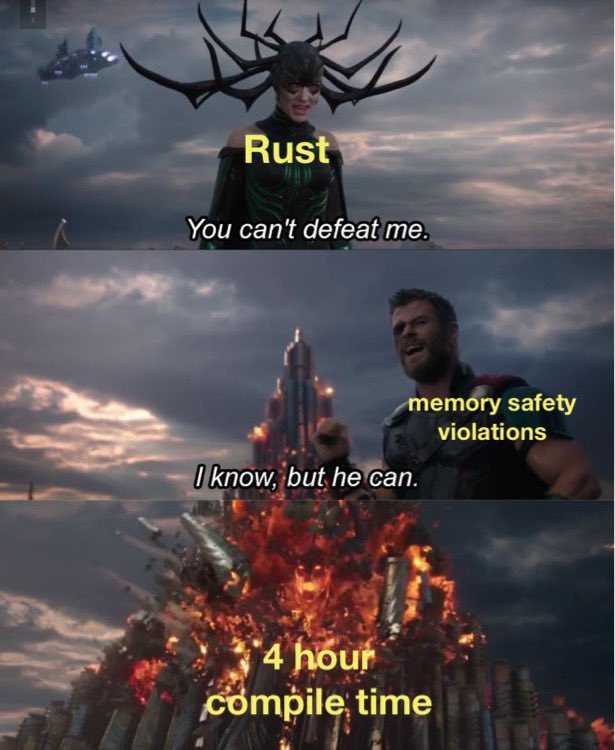
\includegraphics[height=32em]{./images/rust-long-compile-times.jpg}
\captionof{figure}{Rust takes soooooo long to compile. (\citeprocitem{14}{freaker-07, 2023})}
\end{center}

\subsection{Bigger program size}
\label{sec:org0173fb7}
Once again, Rust, being an extremely complex language,
likely will take up more space to ensure that the
safety guarantees offered by the programming language
are enforced. This does pose a problem for programmers
working with embedded systems, like an Arduino,
and Internet of Things (IoT) devices,
as these devices usually have very little storage,
but it is possible to get the Rust compiler to
optimise the program for the tiniest size and
have it work on such devices. It will take more
work on the part of the programmers to optimise their
program, but it is definitely possible to do.  \\

\begin{figure}[htbp]
\centering
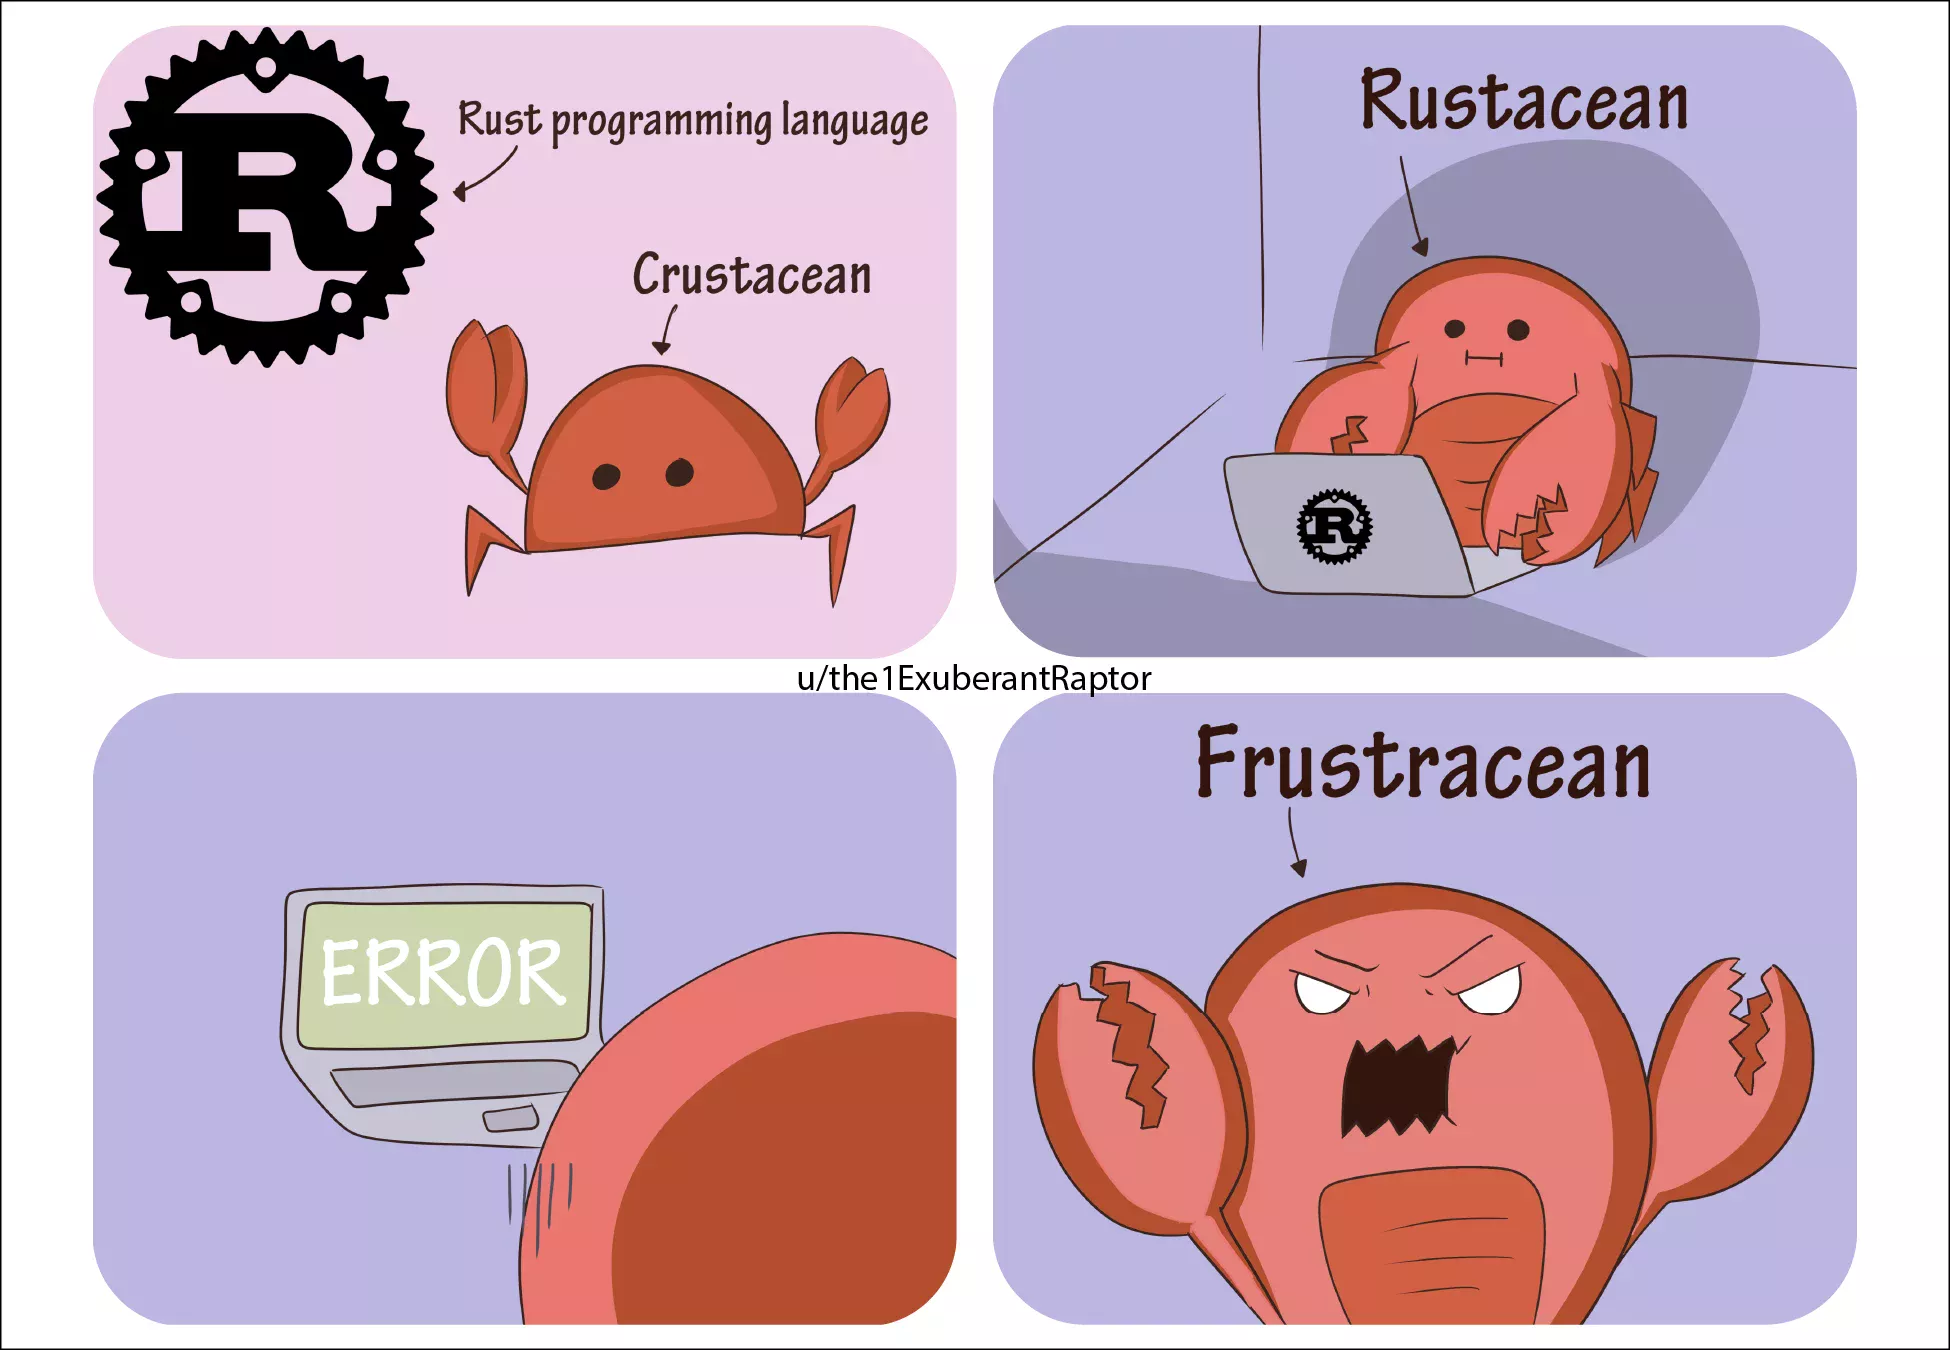
\includegraphics[width=.9\linewidth]{./images/crustacean-rustacean-frustracean.png}
\caption{A meme about programming in Rust. People who program in Rust are known as Rustaceans. (\citeprocitem{37}{the1ExuberantRaptor, 2024})}
\end{figure}

 \newpage

\section{I'm not a programmer, why should I care?}
\label{sec:orgf1e88b9}
\begin{figure}[htbp]
\centering

\includegraphics[height=27em]{./images/why-rust.jpg}
\caption{Why Rust? (\citeprocitem{30}{Rocha, 2018})}
\end{figure}
You should absolutely care about programmers using Rust.
One of the common types of vulnerabilities that are
being exploited by hackers to do all kinds of malicious
things are memory exploitation vulnerabilities.
Google, Microsoft and Mozilla have all reported that
roughly 70\% of all security vulnerabilities are
memory related (\citeprocitem{8}{Chromium, n.d.}; \citeprocitem{17}{Hosfelt, 2019}; \citeprocitem{24}{MSRC, 2019}).
This is especially concerning since all of these
vulnerabilities must have come from memory unsafe
programming languages like C and C++.
Programming languages that make use of a garbage
collector are considered memory safe, as the
memory is automatically managed by the
garbage collector which will not cause
any memory-related bugs if it has been
made correctly, which it usually is.

 \newpage

That must mean that most of these vulnerabilities
are probably used in more critical applications
where performance is of topmost priority, as that
is usually what C and C++ is usually used for.
C and C++ are also used widely in embedded systems
and Internet of Things devices due to the
extremely tight constraints on storage space
and memory size. Most programming languages
that have a garbage collector are just way
too big to run on such devices.
These types of devices are also everywhere,
and some perform critical tasks or contain
extremely private information.
Some examples of such devices are Wi-Fi routers,
security cameras, smart home devices like
smart doorbells and smart locks, smart TVs
and printers.  \\

A malicious actor gaining access to one of these
devices and exploiting a vulnerability to perform
malicious acts, especially a Wi-Fi router or a security
camera, can result in serious damage to you
and your belongings. You may have pictures of you
and your family, your daily routine, and
recordings of intimate moments being leaked
if your security camera was compromised,
resulting in blackmail and possibly burglary,
among other possible crimes. A Wi-Fi router
being compromised could result in all of your
devices being hit with a ransomware attack,
causing huge amounts of data loss if you refuse
to pay the ransom.

\begin{center}

\includegraphics[height=18em]{./images/pull-cables-in-case-of-cyber-attack.jpg}
\captionof{figure}{Effective security I must say. (\citeprocitem{1}{AlooBhujiyaLite, 2023})}
\end{center}

 \newpage

The chances of being hacked are not as low as
you think it is. Staying vigilant online
and not clicking on sketchy links in your browser
does help, along with using an ad blocker,
but that only helps you on your
computer or mobile device. Malicious actors
targetting your Wi-Fi routers or home security
systems don't need you to click on some sketchy
link to hack into those devices and systems,
they will try their utmost to do so without
your input at all. Worst of all, unless you
are actively monitoring and logging the state
of these devices and systems, you likely won't
even know you have been compromised.  \\

Just recently, there was a zero-click vulnerability
affecting Wi-Fi routers and smartphones, with a
Common Vulnerability Scoring System (CVSS) score
of 9.8, which is a critical vulnerability.
This vulnerability affects all Wi-Fi routers
and smartphones that make use of the MediaTek
Wi-Fi chipsets MT7622 and MT7915, as well as
RTxxxx SoftAP driver bundles used in products
from Ubiquiti, Xiaomi and Netgear. The affected
versions include MediaTek SDK versions 7.4.0.1
and earlier, as well as OpenWrt 19.07 and 21.02
(\citeprocitem{26}{News, 2024}; \citeprocitem{33}{Security, 2024}).
Sorry for all that technical detail,
but it is important for you to know
so that you can update your firmware if
you are affected by this vulnerability.

 \newpage

What kind of vulnerability was it? Well, you
guessed it, it was memory-related. Specifically,
the exploit made use of a buffer overflow, which
is when the memory location of the incoming data
is being written to is too small to hold the
entirety of the incoming data. This results in
the incoming data overflowing that memory location,
which results in the data being written
to memory locations outside that initial memory
location. This inevitably allows the malicious
actor to control the memory of a program directly
by changing the content and the size of the input
to the program, which basically allows the
malicious actor to do whatever he wants with
the program, and usually the device as well.
In this case, both were possible.
This is known as remote code execution
or RCE for short, and the malicious actor can do
anything, from changing the password on the
Wi-Fi router to compromise all devices connected
to your network and add them to a botnet,
which is a network of devices a malicious
actor has control over to do his bidding,
usually without the owner or the user of
that device knowing.
The possibilities are endless.

\begin{center}
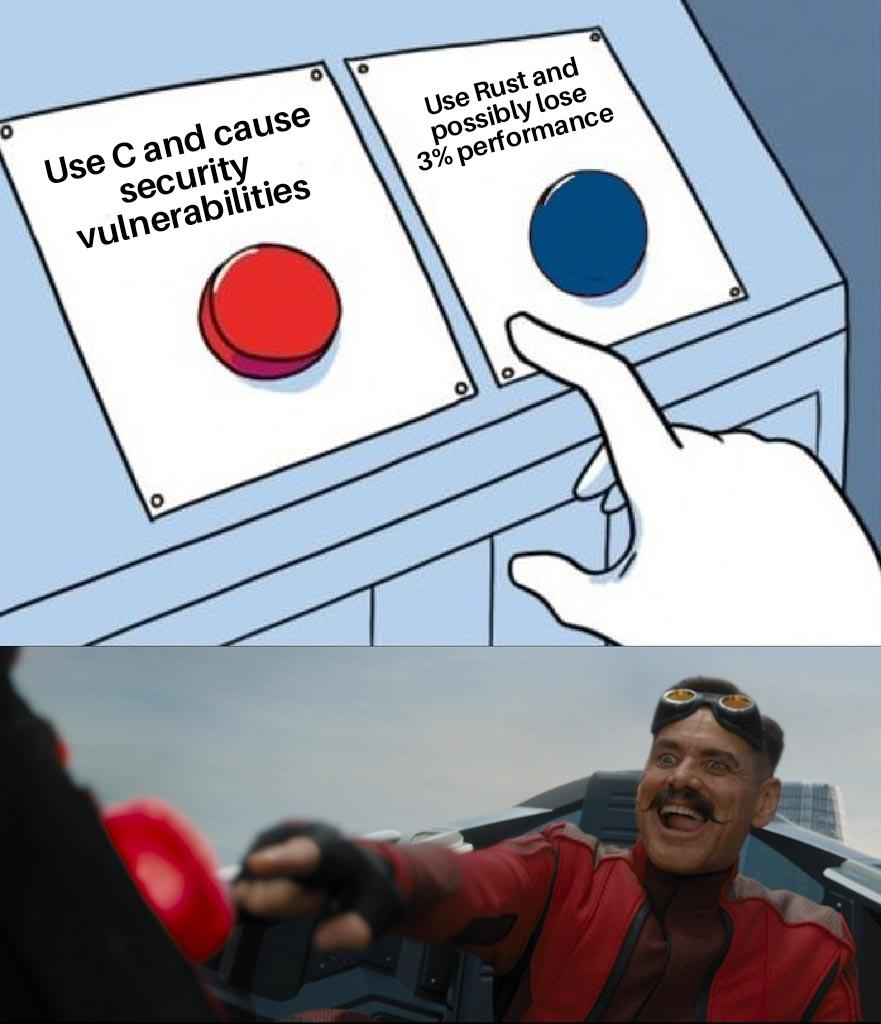
\includegraphics[height=23em]{./images/choosing-c.jpeg}
\captionof{figure}{Well, performance is more important than everything else right? Right? (\citeprocitem{6}{ChipNDipPlus, 2024a})}
\end{center}

 \newpage

As such, it is imperative that more programs are
written in memory-safe languages like Rust to
reduce the occurrence of such severe vulnerabilities.
This is especially the case for embedded and
Internet of Things devices due to their limited
storage space and memory capacity making it impossible
to use other languages with garbage collection.
Programmers who make firmware for these devices
need to use Rust instead of C and C++ to ensure
that such memory-related vulnerabilities
do not occur on their devices.
This way, we can make the internet a safer place for
everyone, and reduce the billions of dollars lost
to cyberattacks yearly. I hope that you also hold
this opinion after reading this blog.  \\

On a more philosophical note,
Jean-Paul Sartre states that writing does not
have an end. A work of art does not have an end
(\citeprocitem{32}{Sartre \& Frechtman, 2012}).
Writing code for software is similar in this regard,
in that it never ends, as it is a form of art after all.
Writing code for a program is never complete,
it is only ever abandoned.
There will always be new features to add,
and new bugs to fix. The Rust programming
language, however, is trying to change that.
With all of its safety guarantees and
language features to reduce the number of
bugs that can occur in a program, we are
slowly inching towards programs that are
truly complete, and will never need another update.
It is currently still a pipe dream for most programmers,
but one can hope that we will eventually
reach a point with a program where it no longer
needs to be updated to work properly,
and has absolutely no bugs, and it seems like
Rust is the programming language that makes it
seem achievable. Hence, every programmer should
learn Rust, write Rust, and improve Rust so that
we will one day no longer need to update our
programs, and still have them work indefinitely.
It seems possible, and seems to be within our reach,
so we should all try to achieve this ultimate goal,
the truly complete program.

 \newpage

\section{Terminology}
\label{sec:orgca2adf1}
Here is just a list of definitions for the
technical jargon used in this blog, in case
you forget what they mean.

\subsection{Memory safety}
\label{sec:org1333ca7}
Memory safety is ensuring that all references
to locations in memory are valid. Valid memory
is memory that has been allocated to the program
and has been initialised with a value.

\subsection{Typecasting (of variables)}
\label{sec:orgb6baa6a}
Typecasting is explicitly changing
the type of a variable to another type,
for example, changing a floating point
number to an integer type.

\subsection{Strongly typed programming language}
\label{sec:org047519e}
A strongly typed programming language
is a programming language that \textbf{does not}
\textbf{implicitly} change a variable's type
from one type to another. You will
have to \textbf{explicitly} change the type
of a variable via type casting. It is usually
most relevant when comparing variables,
but is also relevant when operating on
variables using operators that have
multiple meanings, like \texttt{+}.

\subsection{Compile}
\label{sec:orgd2a7353}
In programming contexts, the process of
converting the code you have written into
machine code that can run on your computer
is called compilation. When a program fails
to compile, it means that this conversion
process from the code you have written
into machine code has failed.

\subsection{Float (floating point number)}
\label{sec:org05a1ad0}
A floating point number, or float,
is just a number that has decimal places
in programming languages.
The name has a good reason behind it, but
it is unnecessary for you to know, and
is very technical, which will likely bore you.

\subsection{Integer}
\label{sec:org5517943}
An integer is basically a whole number,
with no decimal places.

\subsection{String}
\label{sec:orgf4370b9}
A string in programming languages is just text,
usually enclosed in single ('') or double
quotes ("").

\subsection{Statically typed programming language}
\label{sec:org0af6b10}
A statically typed programming language
is a programming language that \textbf{does not}
allow you to change the type of a variable
after creating it. If you want to change
the type of a variable via type casting,
you will have to store the result of that
type cast in another variable. You can't
use the same variable again to store
the result of the typecasting.

\subsection{General-purpose programming language (GPL)}
\label{sec:org42c1d6a}
A general-purpose programming language is
a programming language that can be easily used
to do pretty much whatever you want it to do.
Some examples include Python, Java, C, C++ and Rust.

\subsection{Function}
\label{sec:org0c1d2ba}
A function in programming refers to the same
concept in mathematics. It is something
that takes some input and returns an output.
In programming contexts, functions usually
do useful things and allow you to use
them anywhere you want after you have
written them, so you don't have to write
the same code over and over again to do
the same thing.

 \newpage

\subsection{Library}
\label{sec:org789d0e9}
A library in the programming context refers to
pre-made code that is a collection of
useful functions that you can use to make
writing your program faster and easier,
as you won't need to write all the functions
you need yourself, and can just use the
functions other people have written.

\subsection{Domain-specific language (DSL)}
\label{sec:org826fce1}
A domain-specific language is a language
(not necessarily a programming language,
HTML is a markup language,
not a programming language) that is used
for a very specific purpose, like scientific
computing (R and MATLAB),
or manipulating databases (SQL).

\subsection{Garbage collector}
\label{sec:org096bea1}
A garbage collector is a process that runs separately
from the main program that cleans up unused references
to free the memory used for other programs on
your computer to use.

\subsection{Pointers / References}
\label{sec:orgd14daf4}
Pointers and references are
simply a memory address,
and that memory address refers to a
place in memory that contains some useful
information so that the program knows
where to find the information stored.

 \newpage

\subsection{Low-level programming language}
\label{sec:orgf0afedc}
A low-level programming language is a programming language
that allows you to manipulate memory directly by using
pointers.

\subsubsection{Comment}
\label{sec:org490cbda}
The definition of low-level programming languages
has changed quite a lot as pretty much all programming
languages are considered high-level languages, even C
and C++.  \\

Truly low-level programming languages like assembly and machine code
are no longer the standard for what is considered low-level,
as very few people use them and the definition is just not
very relevant or useful in modern times.

\subsection{Memory leak}
\label{sec:org5127c78}
A memory leak refers to the situation where a program uses up
some memory, but fails to release that memory after it
is done with the memory. This usually happens due to
programmers forgetting to free the memory used by a
variable in low-level languages like C and C++.
This results in the program hogging memory for
no reason, as it is already done with the memory,
but just didn't release it back for other programs to use.  \\

It is called a "leak" because the program doesn't have any
control over the memory that it is done using
and was supposed to be released. That memory has escaped
the control of the program and has "leaked" into the
rest of the system. The program can no longer release
the memory back to the system, even if it wanted to,
which means the program will slowly use up more and
more memory until the system crashes due to running out
of memory. Memory leaks are notoriously difficult
to catch and debug as they are usually not noticeable
until the system crashes out of nowhere after running
the program for a very long time.

\subsection{Scope}
\label{sec:org4b5fb86}
A scope in the programming context is quite abstract
and can be difficult to explain properly, but
for this blog, all you need to know is that a
scope in the Rust programming language is the
code inside a pair of curly braces (\texttt{\{\}}) that
is \textbf{not} inside single ('') or double quotes ("").

\subsection{Function signature}
\label{sec:org989e263}
A function signature describes a function written
in a program. It tells you the parameters of the
function, which is what you need to give as input
into the function, and its return type, which is
the function's output.

\subsection{Body of a function (function body)}
\label{sec:org8772366}
The function body is the place where the code
for what the function does is written.

\subsection{Implementation of a function}
\label{sec:org8f21de3}
The implementation of a function refers to the
body of the function. There are many ways
to do the same thing in programming, so the
implementation of one function by two different
people can be entirely different.

\subsection{Mutability}
\label{sec:orgec4d1bb}
Mutability refers to being able to change something.
In the programming context, it usually refers to variables.

\subsection{Compiler}
\label{sec:org249d3a1}
A compiler is a program that turns the code
written in a programming language to machine code
so that it can be run on your computer.

\subsection{Enumeration (enum)}
\label{sec:org1746d9b}
An enumeration is just a type that contains a set
of values with names to easily refer to the values.

\subsection{Vulnerability}
\label{sec:orgf561686}
A vulnerability is usually just a bug in a program,
but the bug allows a malicious actor, like a hacker
to make use of that bug to do malicious things
to a device.

\subsection{Compromise}
\label{sec:orgcc15205}
Compromised in the cybersecurity context just means
you got hacked.

\subsection{Botnet}
\label{sec:orga66d3a2}
A botnet is usually a massive network of devices
that is under the control of a malicious actor.
These devices can be used to do anything the
malicious actor wants, and usually without the
owner or the user of those devices knowing.

\subsection{Buffer overflow}
\label{sec:orgfceda3d}
A buffer overflow is a memory bug that occurs when
the memory location that the incoming data is being
written to is too small to hold the incoming data.
The incoming data then overflows that memory location
and starts being written to other locations in memory.
This results in the incoming data being able to
directly control the memory of the program by
changing the size and content of the data, and
it usually results in a pretty severe vulnerability.

\subsection{Remote code execution (RCE)}
\label{sec:org490dffc}
Remote code execution means a malicious actor from
anywhere in the world can remotely execute
code on your device. It is usually considered
a \textbf{critical} vulnerability as this allows the
malicious actor to do literally whatever he wants
with your device.

 \newpage

\section{Bibliography}
\label{sec:org699e259}
Below is the list of references used in this blog:  \\

\begin{hangparas}{1.5em}{1}
\hypertarget{citeproc_bib_item_1}{AlooBhujiyaLite. (2023). R/programmerhumor on reddit: Security++. In \textit{Reddit}. \url{https://reddit.com/r/ProgrammerHumor/comments/13oapsk/security/}}

\hypertarget{citeproc_bib_item_2}{BabuShonaMuhMeLoNa. (2021). R/programmerhumor on reddit: Garbage collector knows. In \textit{Reddit}. \url{https://reddit.com/r/ProgrammerHumor/comments/nkjm6i/garbage_collector_knows/}}

\hypertarget{citeproc_bib_item_3}{Bayer, C. (2017). R/programmerhumor on reddit: Strong typing. In \textit{Reddit}. \url{https://reddit.com/r/ProgrammerHumor/comments/6xfdzr/strong_typing/}}

\hypertarget{citeproc_bib_item_4}{Binstock, A. (2015). Oracle brandvoice: Java’s 20 years of innovation. In \textit{Forbes}. Forbes Magazine. \url{https://www.forbes.com/sites/oracle/2015/05/20/javas-20-years-of-innovation/}}

\hypertarget{citeproc_bib_item_5}{Bit48. (2021). R/programmerhumor on reddit: Why doesn’t c++ have a garbage collector? In \textit{Reddit}. \url{https://reddit.com/r/ProgrammerHumor/comments/qg9xtv/why_doesnt_c_have_a_garbage_collector/}}

\hypertarget{citeproc_bib_item_6}{ChipNDipPlus. (2024a). R/rustjerk on reddit: Can’t argue with that! In \textit{Reddit}. \url{https://reddit.com/r/rustjerk/comments/1drxeai/cant_argue_with_that/}}

\hypertarget{citeproc_bib_item_7}{ChipNDipPlus. (2024b). R/rustjerk on reddit: Gotta ask.. In \textit{Reddit}. \url{https://reddit.com/r/rustjerk/comments/1dtmif8/gotta_ask/}}

\hypertarget{citeproc_bib_item_8}{Chromium. (n.d.). In \textit{Memory safety}. \url{https://www.chromium.org/Home/chromium-security/memory-safety/}}

\hypertarget{citeproc_bib_item_9}{corianderL. (2020). R/rustjerk on reddit: Rust when you use unsafe. In \textit{Reddit}. \url{https://reddit.com/r/rustjerk/comments/ep5oti/rust_when_you_use_unsafe/}}

\hypertarget{citeproc_bib_item_10}{Daniel. (2023). Ownership and borrowing in rust - data engineering gold mine. In \textit{Confessions of a data guy}. Daniel. \url{https://www.confessionsofadataguy.com/ownership-and-borrowing-in-rust-data-engineering-gold-mine/}}

\hypertarget{citeproc_bib_item_11}{ElyeProj. (2022). R/programmerhumor on reddit: I hope some “languages” have more compile-time errors. In \textit{Reddit}. \url{https://reddit.com/r/ProgrammerHumor/comments/vuq1h1/i_hope_some_languages_have_more_compiletime_errors/}}

\hypertarget{citeproc_bib_item_12}{fnabinash. (2024). R/programmerhumor on reddit: rustisblazinglyfast. In \textit{Reddit}. \url{https://reddit.com/r/ProgrammerHumor/comments/1fp78tp/rustisblazinglyfast/}}

\hypertarget{citeproc_bib_item_13}{Forgotten\_Who. (2020). R/programmerhumor on reddit: Garbage collection. In \textit{Reddit}. \url{https://reddit.com/r/ProgrammerHumor/comments/k74xk4/garbage_collection}}

\hypertarget{citeproc_bib_item_14}{freaker-07. (2023). R/programmerhumor on reddit: Uh, oh.. In \textit{Reddit}. \url{https://reddit.com/r/ProgrammerHumor/comments/133kj2y/uh_oh/}}

\hypertarget{citeproc_bib_item_15}{GkAm1. (2021). R/programmerhumor on reddit: Now we are all “string”. In \textit{Reddit}. \url{https://www.reddit.com/r/ProgrammerHumor/comments/mk2wq7/now_we_are_all_string/}}

\hypertarget{citeproc_bib_item_16}{GreekCSharpDeveloper. (2021). R/rustjerk on reddit: Rust programmers are clearly superior. In \textit{Reddit}. \url{https://reddit.com/r/rustjerk/comments/p38bxx/rust_programmers_are_clearly_superior}}

\hypertarget{citeproc_bib_item_17}{Hosfelt, D. (2019). Implications of rewriting a browser component in rust – mozilla hacks - the web developer blog. In \textit{Mozilla hacks – the web developer blog}. \url{https://hacks.mozilla.org/2019/02/rewriting-a-browser-component-in-rust/}}

\hypertarget{citeproc_bib_item_18}{ItsCaptainS. (2022). R/programmerhumor on reddit: No garbage collector. In \textit{Reddit}. \url{https://reddit.com/r/ProgrammerHumor/comments/xyofcd/no_garbage_collector/}}

\hypertarget{citeproc_bib_item_19}{K4r4kara. (2020). R/rustjerk on reddit: Rust lifetimes make me want to end my lifetime. In \textit{Reddit}. \url{https://reddit.com/r/rustjerk/comments/i8gys8/rust_lifetimes_make_me_want_to_end_my_lifetime/}}

\hypertarget{citeproc_bib_item_20}{Kelley, A. (2016). Introduction to the zig programming language. In \textit{Introduction to the zig programming language - andrew kelley}. \url{https://andrewkelley.me/post/intro-to-zig.html}}

\hypertarget{citeproc_bib_item_21}{LinearArray. (2024). R/rustjerk: In rust we trust \&lt;3. In \textit{Reddit}. \url{https://reddit.com/r/rustjerk/comments/1c3dnga/in_rust_we_trust_3}}

\hypertarget{citeproc_bib_item_22}{Migala, J. (2018). What do you get from a banana? plus answers to 8 other questions. In \textit{Everydayhealth.com}. \url{https://www.everydayhealth.com/diet-nutrition/diet/what-you-get-from-banana-plus-answers-other-questions/}}

\hypertarget{citeproc_bib_item_23}{mottosson. (2021). R/rustjerk on reddit: It’s unsafe to go alone.. In \textit{Reddit}. \url{https://reddit.com/r/rustjerk/comments/q1fg7x/its_unsafe_to_go_alone/}}

\hypertarget{citeproc_bib_item_24}{MSRC. (2019). Microsoft. In \textit{Msrc blog | microsoft security response center}. \url{https://msrc.microsoft.com/blog/2019/07/a-proactive-approach-to-more-secure-code/}}

\hypertarget{citeproc_bib_item_25}{navierstokes88. (2023). R/programmerhumor on reddit: rust devs in a nutshell. In \textit{Reddit}. \url{https://reddit.com/r/ProgrammerHumor/comments/1129u2y/rust_devs_in_a_nutshell/}}

\hypertarget{citeproc_bib_item_26}{News, S. (2024). Critical exploit in mediatek wi-fi chipsets: Zero-click vulnerability (cve-2024-20017) threatens routers and smartphones. In \textit{Sonicwall}. Security News https://blog.sonicwall.com/wp-content/uploads/images/logo/SonicWall\_Registered-Small.png. \url{https://blog.sonicwall.com/en-us/2024/09/critical-exploit-in-mediatek-wi-fi-chipsets-zero-click-vulnerability-cve-2024-20017-threatens-routers-and-smartphones/}}

\hypertarget{citeproc_bib_item_27}{OOLarge. (2019). R/programmerhumor on reddit: I’ve been dealing with memory leaks at work. In \textit{Reddit}. \url{https://reddit.com/r/ProgrammerHumor/comments/b9uh5z/ive_been_dealing_with_memory_leaks_at_work/}}

\hypertarget{citeproc_bib_item_28}{richardanaya. (2022). R/rustjerk on reddit: Ferris subverted the true mascot of the rust programming language. respect the fungus. In \textit{Reddit}. \url{https://reddit.com/r/rustjerk/comments/w8ssrp/ferris_subverted_the_true_mascot_of_the_rust/}}

\hypertarget{citeproc_bib_item_29}{Ritchie, D. M. (1993). The development of the c language. \textit{Acm Sigplan Notices}, \textit{28}(3), 201–208. \url{https://doi.org/10.1145/155360.155580}}

\hypertarget{citeproc_bib_item_30}{Rocha, B. (2018). Rochacbruno/rust\_memes: The best memes and stickers about \#rust \#rustlang - listed here for easy use on talks and share. In \textit{Github}. \url{https://github.com/rochacbruno/rust_memes}}

\hypertarget{citeproc_bib_item_31}{Rossum, G. v. (1991). In \textit{Python 0.9.1 part 01/21}. \url{https://www.tuhs.org/Usenet/alt.sources/1991-February/001749.html}}

\hypertarget{citeproc_bib_item_32}{Sartre, J.-P., \& Frechtman, B. (2012). \textit{What is literature?} Philosophical Library/Open Road.}

\hypertarget{citeproc_bib_item_33}{Security, C. (2024). 4 Exploits, 1 bug: Exploiting cve-2024-20017 4 different ways. In \textit{Hyprblog}. \url{https://blog.coffinsec.com/0day/2024/08/30/exploiting-CVE-2024-20017-four-different-ways.html}}

\hypertarget{citeproc_bib_item_34}{SirKastic23. (2023). R/rustjerk on reddit: Why?? In \textit{Reddit}. \url{https://reddit.com/r/rustjerk/comments/16mhgf6/why/}}

\hypertarget{citeproc_bib_item_35}{Skills, R. (2022). Solidity the weird parts. In \textit{Youtube}. YouTube. \url{https://www.youtube.com/watch?v=UX-4rAXFvWw}}

\hypertarget{citeproc_bib_item_36}{StBlaize. (2024). R/programmerhumor on reddit: theexception. In \textit{Reddit}. \url{https://reddit.com/r/ProgrammerHumor/comments/1egqw3x/theexception/}}

\hypertarget{citeproc_bib_item_37}{the1ExuberantRaptor. (2024). Rust programming language. In \textit{Coding memes}. \url{https://www.codeitbro.in/programming-memes/rust-programming-language/}}

\hypertarget{citeproc_bib_item_38}{TheONEO. (2021). R/programmerhumor on reddit: Why do you say my program has a memory leak? In \textit{Reddit}. \url{https://reddit.com/r/ProgrammerHumor/comments/p3o441/why_do_you_say_my_program_has_a_memory_leak/}}

\hypertarget{citeproc_bib_item_39}{TheoXDM. (2022). R/programmerhumor on reddit: Exception e. In \textit{Reddit}. \url{https://reddit.com/r/ProgrammerHumor/comments/zsuj9u/exception_e}}

\hypertarget{citeproc_bib_item_40}{Thompson, C. (2023). How rust went from a side project to the world’s most-loved programming language. In \textit{Mit technology review}. MIT Technology Review. \url{https://www.technologyreview.com/2023/02/14/1067869/rust-worlds-fastest-growing-programming-language/}}

\hypertarget{citeproc_bib_item_41}{valchap. (2023). R/rustjerk on reddit: The borrow checker in a nutshell. In \textit{Reddit}. \url{https://reddit.com/r/rustjerk/comments/17211ks/the_borrow_checker_in_a_nutshell/}}

\hypertarget{citeproc_bib_item_42}{Vijay. (2024). R/programmerhumor on reddit: whatisadomainspecificlanguage. In \textit{Reddit}. \url{https://redlib.nohost.network/r/ProgrammerHumor/comments/1e9sn0b/whatisadomainspecificlanguage}}

\hypertarget{citeproc_bib_item_43}{Wikipedia. (2024a). In \textit{Wikipedia}. Wikimedia Foundation. \url{https://en.wikipedia.org/wiki/C\%2B\%2B}}

\hypertarget{citeproc_bib_item_44}{Wikipedia. (2024b). In \textit{Wikipedia}. Wikimedia Foundation. \url{https://en.wikipedia.org/wiki/Rust_(programming_language)}}

\hypertarget{citeproc_bib_item_45}{Wikipedia. (2024c). In \textit{Wikipedia}. Wikimedia Foundation. \url{https://en.wikipedia.org/wiki/Go_(programming_language)}}

\hypertarget{citeproc_bib_item_46}{Wilcke, K. (2023). R/programmerhumor on reddit: Static vs dynamic typing by the great kolja wilcke. In \textit{Reddit}. \url{https://www.reddit.com/r/ProgrammerHumor/comments/12q3lhb/static_vs_dynamic_typing_by_the_great_kolja_wilcke/}}\bigskip
\end{hangparas}
\end{document}
